\begin{chapter}{A Decision Support Framework for Offshore Wind \label{Ch:ds-for-ow}}

Consider the problem of storing spare subassemblies, which will replace subassemblies in an offshore wind farm which have suffered a `serious' failure. Spare parts may be stored in a warehouse near to the dock, at which spare parts will be loaded onto a boat so the spare can be shipped out to the turbine to be fitted. This problem has been considered previously in the literature. \citet{Tracht2013} perform a scenario analysis which investigates the effect of limited amounts of spare components and equipment on preventative maintenance. A review of various models used for analysing spare parts strategies is given in \citet{Tusar2022}. The review stresses that not enough work is being done on constructing an optimal combination of spare parts, as once an order has been placed, the time to delivery for spare components can be sufficiently long to reduce availability. We aim to address this. The review suggests most analyses are interested in minimising downtime. Our analysis will consider availability (downtime is essentially the opposite of availability) but we will also consider the costs incurred by increasing availability.

This chapter proposes a decision support framework which is flexible enough to incorporate relevant sources of uncertainty into a decision support exercise. A key difference with our approach, compared to standard approaches, will be that we use ideas from the history matching (HM) and BayesOpt literature to construct a set of sensible decisions. BayesOpt is typically used to find a single decision which is (approximately) optimal, but the BayesOpt routine also provides us with an emulator across the entire decision space, which can be used to construct a set of feasible decisions. Our approach is novel as we will employ ideas from HM to conduct a post-hoc analysis of the BayesOpt routine.

We will begin by outlining competing objectives a DM may consider in an offshore wind setting. We progress to formalising the decision problem and thus translating the decision problem to an optimisation problem. A novel application of BayesOpt and HM techniques then allows us to construct a set of sensible decisions; the DM will be presented with this set and uses it to make a final decision.
\section{The decision problem}

Recall that the Athena simulator models a turbine as being composed of $8$ important subassemblies, and a ninth `catch all' subassembly. They are as follows: 1. gearbox, 2. generator, 3. frequency converter, 4. transformer, 5. main shaft bearing, 6. blades, 7. tower, 8. foundations, and 9. catch all. The DM has two problems to solve simultaneously, whilst aiming to maintain high availability of the wind farm:
\begin{itemize}
 \item[1.] Which warehouse, from a set of candidate warehouses, should the spare parts be stored in?
 \item[2.] What is the best way to manage the warehouse?
\end{itemize}
Good management of a sub-optimal warehouse may be much better than bad management of the optimal warehouse. Of course, we strive for optimal management of the optimal choice of warehouse. The management of the warehouse is broken down into the answers of the following two questions:
\begin{itemize}
 \item[1.] How many spare parts should we store for each subassembly?
 \item[2.] At what point should we buy in more spare parts for the subassembly?
\end{itemize}
%Almost every problem so far in this thesis has been addressed with decision theory. That theme is not going to end on page \thepage.
We therefore need to formulate a utility function over all relevant attributes and specify an appropriate prior distribution over uncertain quantities. We do not directly specify any particular prior distribution; we instead adopt the priors elicited by \citet{Zit2021}. These priors were elicited from practising engineers who are able to give informed assessments of uncertain quantities. We will act as the DM as well as the analyst. In this exercise we will specify the utility function. The utility function will express sensible preferences, but will not represent the preferences of a real DM. We stress that the emphasis of this chapter is the development of an appropriate optimisation/decision support framework, rather than precise details of utility functions or precise details of the problem itself.

\section{Mathematical formulation of the decision problem}
Here we will formulate the decision problem following the elicitation guidelines outlined in \cref{Ch:background}; more details can be found in \citet{Smith2010} or \citet{Keeney1976}. Our problem is to choose a warehouse, $k$, of size $W_k$, and fill the warehouse with spare parts for each of the $9$ subassemblies. We will allocate $s_i$ spares for subassembly $i$. We also need to construct a policy for restoring the numbers of spare parts as they deplete, to ensure smooth running of the warehouse.

We begin by identifying an appropriate set of attributes. We then specify preferences through marginal utility functions, which will be combined into a single multi-attribute utility function. The first stage of elicitation of a utility function is to define all attributes relevant to the problem.

\subsubsection{Relevant attributes}

There are several attributes relevant to this problem. The key attributes are:
\begin{itemize}
 \item The availability time series (performance) of the wind farm.
 \item The choice and cost of the warehouse in which spare parts are stored.
 \item The number of spares of each type of subassembly.
 \item The policy which dictates when to buy in more spare parts.
\end{itemize}
There are many more attributes a DM could consider, but this is sufficient in our case to demonstrate the complexity of the problem and the application of methodology. We would next need to decide what the consequences, $c_i$, of any possible decision would be. The consequences of any decision are given in \cref{Tab:consequences} alongside information about the consequences. For example, the availability time series output by Athena over a $5$ year period is internally processed by Athena and a length $240$ vector is output. We know that this time series is stochastic. The restoration policy is both a decision and a consequence here; the consequence is the set of $p_i$, the thresholds that trigger an ordering for more spare parts of type $i$ as in \cref{Sec:athena-variant}, we would want to leave this as late as possible. The cost of the warehouse could be argued to be stochastic (for example, if the unit is rented, the owner may increase the rent to some uncertain value at some uncertain future time point). We assume, for simplicity, that the cost is fixed and related to its capacity. In \cref{Tab:consequences} we the use notation $\mathcal{S}^k_n$. This represents the $k$ dimensional discrete simplex which we will define as
\begin{equation}
 \mathcal{S}^k_n = \left\{\bx \in \N^{k+1} \,\,\bigg|\, \sum_{i=1}^{k+1} x_i = n, x_i \in \{1, 2, \ldots, n-k+1\} \right\}. \label{Eq:disc-simplex}
\end{equation}
We have chosen to define $\mathcal{S}^k_n$ in this way as it reflects aspects of our application. A warehouse of size $n$ can have a minimum of $1$ spare part of type $i$ and can have at most $n-k+1$ spare parts of type $i$. This is because the other $k-1$ types of component all need at least $1$ spare part. This essentially assumes that all spare subassemblies are of similar shape and size, this is clearly an over simplification which could be addressed in future work.

%decisions
\begin{table}[t]
	\centering
	\begin{tabular}{llll}
		\toprule
  Label & Description & Parameter Space & Stochastic?\\\cmidrule{1-4}
  $c_1$ & Availability time series & $c_1 \in (0, 1)^{240}$& Yes\\
  $c_2$ & Choice of the restoration policy &$c_2 \in (1, 99)^9$& No\\
  $c_3$ & Warehouse size & $c_3 \in \{50, 75, 100\}$& No\\\bottomrule
	\end{tabular}
	\caption{Summary of the consequences of a future decision to be made. These variables cause changes in the stochastic and deterministic consequences and it is the decisions themselves that will form the inputs of a future emulator.	The stochastic column describes how we model the consequence. \label{Tab:consequences}}
\end{table}
%consequences
\begin{table}[t]
	\centering
	\begin{tabular}{lll}
		\toprule
  Label & Description & Parameter Space\\\cmidrule{1-3}
  $x_1$--$x_9$ & Number of spare parts & $x_{1:9} \in \mathcal{S}^{8}_{x_{19}}$\\
  $x_{10}$--$x_{18}$ & Critical Percentages & $x_{10:18} \in (1,99)^9$\\
  $x_{19}$ & Warehouse size (number of parts) & $x_{19} \in \{ 50, 75, 100 \}$\\\bottomrule
	\end{tabular}
	\caption{Summary of the decision variables. These are the variables for which individual utility functions will be elicited, to be combined into an overall utility function. See \cref{Eq:disc-simplex} for the definition of $\mathcal{S}^k_n$.	\label{Tab:consequences}}
\end{table}
Our approach to eliciting the utility function will follow the advice of \citet{Smith2010} and \citet{Keeney1976}. We assume that consequences are mutually utility independent, elicit a marginal utility function for each consequence using probability or certainty equivalents and then combine the marginal utility functions into an overall utility function via a multiplicative or additive form, depending on the preferences of the DM.
\section{The marginal utility functions}
Utility functions are unique up to positive affine transformations. That is, $au(x) + b$ expresses exactly the same preferences as $u(x)$ for any $a > 0$ and $b \in \R$. For this reason, we will construct all utility functions on the unit interval. This also allows for easier elicitation, as utility and probability will be on the same scale.
\subsubsection{Utility of availability}
The availability is a time series. At time $t$, denote the (random) availability by $A(t)$, this will form our first consequence. In particular, the Athena simulator outputs a length $L$ time series, $(A(t_1), A(t_2), \ldots, A(t_{L}))$ at equally spaced intervals. In our analysis, $L = 240$ due to various settings within Athena. We therefore define $c_1(t) = A(t)$ and let $c_1 = (c_1(t_1), c_1(t_2), \ldots, c_{1}(t_{L}))$. The utility of a time series may be time dependent, however, in this problem we will work with the assumption that a given availability has utility which does not depend on time. In other words, if we let $\tilde{u}_1(c_1(t), t)$ be the utility for $c_1(t)$ at time $t$ then $\tilde{u}_1(c_1(t), t) = \tilde{u}_1(c_1(t))$. We would then take the utility of the entire time series to be
\begin{equation}
 u_1(c_1) = \frac{1}{L}\sum_{j = 1}^{L} \tilde{u}_1(c_1(t_j)).
\end{equation}
This is just point-wise utility averaged over time. This average could be weighted if high availability is more important at some time points than others. See \citet{Rios2003} for examples of time-dependent utility elicitation.

We believe a utility function which allows for a varying attitude to risk would be appropriate for $\tilde{u}_1(c_1(t))$. The reason for this is that, for regions of high availability, a DM would be risk-averse, or risk-neutral, in trying to increase availability. However, whenever the availability is very low, we would be risk-seeking in order to ensure the wind farm is viable. An appropriate functional form is:
\begin{equation}
 \tilde{u}_{1}(c) = \beta^{-1} \left\{\frac{(c - a)}{\sqrt{1 + b (c-a)^2}} - \alpha\right\}
\end{equation}
where $a \in (0,1)$ and $b>0$ are parameters to be elicited and $\alpha$, $\beta \in \R$ are scaling parameters which force $0 \leq \tilde{u}_{1}(c) \leq 1$ for any $c \in [0,1]$. $\alpha$ and $\beta$ have the following algebraic forms:
\begin{align}
 \alpha &= -\frac{a}{\sqrt{1 + a^2b}}\\
 \beta &= \frac{1 - a}{\sqrt{1 + b(1-a)^2}} -\frac{a}{\sqrt{1 + a^2b}}.
\end{align}
Now, since we enforce the constraints $\tilde{u}_1(0) = 0$ and $\tilde{u}_1(1) = 1$, we only need to elicit two certainty equivalents to construct a fitted form for $u_1(c)$. To do this, we will use a bisection method. First we specify the availability, $c^{(1)}$, such that $[0, 1; 0.5] \sim c^{(1)}$ then we specify $c^{(2)}$ such that $[c^{(1)}, 1; 0.5] \sim c^{(2)}$. These certainty equivalences imply $\tilde{u}_1(c^{(1)}) = 0.5$ and $\tilde{u}_1(c^{(2)}) = 0.75$. We therefore have two equations in two unknowns which can be solved for $(a , b)$ (and thus $\alpha$ and $\beta$ are also found). The chosen values were $u_1(0.9)= 0.5$ and $u_1(0.95) = 0.75$ which implies $(a, b) = (0.95, 50)$. To validate the utility function, we could ask for $c^{(3)}$ such that $\tilde{u}_1(c^{(3)}) = 0.25$. We would then compare the value of $c$ which gives $\tilde{u}_1(c) = 0.25$ to the elicited $c^{(3)}$. An illustration of the fitted $\tilde{u}_1(c_1)$ is given in \cref{Fig:u1-c1}. We see that when $c_1 < 0.9$, we have risk-seeking behaviour, for $c_1 \geq 0.9$, the behaviour is approximately risk-neutral.
\begin{figure}
 \centering
 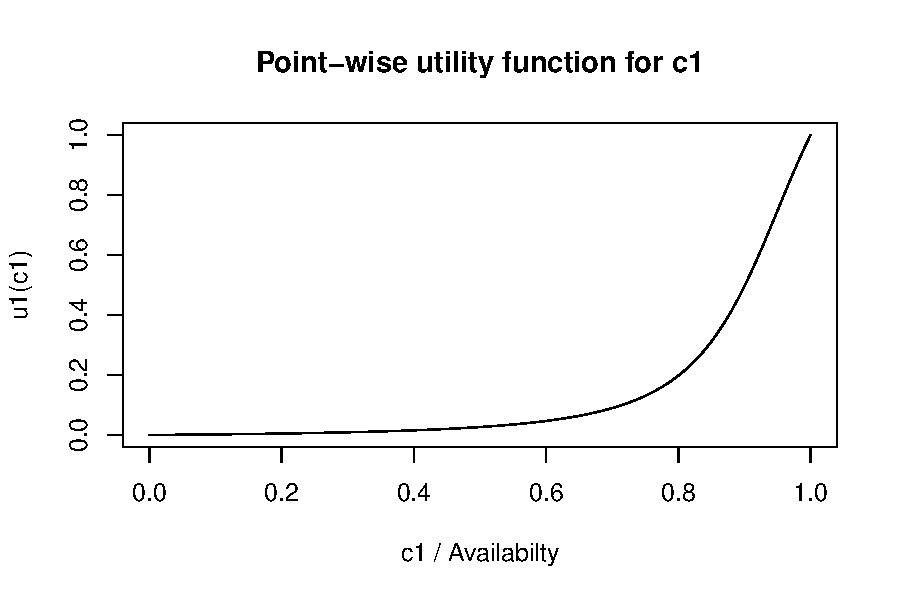
\includegraphics{fig-ds/u1-c1.pdf}
 \caption{Plot of the fitted utility function for point-wise availability; $\tilde{u}_1(c_1)$.\label{Fig:u1-c1}}
\end{figure}
\subsubsection{Utility of warehouse size}
We assume that the smallest warehouse possible is preferred, as this will likely be cheaper. The sizes of the warehouses are $\{50, 75, 100\}$, thus we need $u_2(100) = 0$ and $u_2(50) = 1$. Since the warehouses are discrete decisions, and there are only three warehouses in our problem, it may be better to simply elicit a value for $u_2(75)$ than specify a utility function. However, this would not allow for feedback or analysis of risk aversion. We propose using a risk averse utility function for this part of the problem. A simple, risk averse, form is
\begin{equation}
 u_2(c_2) = 1 - \left(\frac{c_2 - a}{b - a}\right)^2
\end{equation}
where $(a, b)$ are constants to ensure $u(50) = 1$ and $u(100) = 0$. For this problem we have $a = 50$ and $b = 100$. We could then ask the DM what their utility for $c_2 = 75$ is and compare to the value $u_2(75) = 0.75$. We could also try other functional forms. However, since this is an extended illustrative example, we settle on
\begin{equation}
 u_2(c_2) = 1 - \left(\frac{c_2 - 50}{50}\right)^2
\end{equation}
as it reflects realistic beliefs about the problem whilst retaining simplicity.
\subsubsection{Utility of spares restoration}
When spares are restored, we aim to fill up the initial allocation of spares for that particular type of component. We adopt a policy that reflects that spares should be restored as late as possible, without adversely affecting availability. Our utility function should then reflect that restoring the numbers of spares happens as late as possible. Let the number of remaining spare parts for subassembly $i$ be $s_i (t)$ (which from hereon in will be implicitly a function of time). One way to specify when spares are restored is to specify a value $s'_i$ for the $i$th subassembly such that, at the instant when $s_i < s'_i$ is first satisfied, an order for more spare parts is placed. We would like to avoid having a utility function which depends on another decision, since $s'_i \leq s_i$. We can instead express this decision as an independent attribute by finding the proportion of spares, $p_i$ such that when $\frac{s_i}{s'_i} < p_i$ more spares must be ordered, where $p_i \in (1, 99)\%$ is the `critical percentage' for ordering more spares. This phrasing of the problem in terms of proportions has two advantages. It makes specifying the utility function easier, as the proportion and the number of spares are independent attributes. Additionally, maximising $U(\bx)$ when there is a complex dependence structure between elements of $\bx$ will be difficult.

Therefore, the third set of decision variables will be $x_{10:18} = (p_1, p_2, \ldots, p_9)$. The following utility function is an appropriate choice for the restoration policy for the $j$th spare component
\begin{equation}
 u_{3,j}(c_{3,j}) = 1 - \left(\frac{1 - c_{3, j}}{99 - 1}\right)^2
\end{equation}
which is a risk-averse utility function which decreases as $c_{3, j} = x_{j+9}$ increases. To combine this into an overall utility function for the spares restoration policy, we could construct a weighted average
\begin{equation}
 u_3 (c_3) = \sum_{j = 1}^9 k_j u_{3,j}(c_3).
\end{equation}
To elicit the weights, $k_j$, we can apply standard multi-attribute elicitation techniques, such as those in \citet{Gonzalez2018}. We however have no preference for one type of spare over another, hence we take $k_j = \frac{1}{9}$ for all $j$. This results in the utility function for $c_3$ being
\begin{equation}
 u_3(c_3) = 1 - \frac{1}{9}\sum_{j=1}^9 \left(\frac{1 - c_{3, j}}{98}\right)^2.
\end{equation}
\subsubsection{Combining all attributes}
To combine the attributes we will use a probability equivalence
 approach \citep{Gonzalez2018}. Recall that $c^{*}$ is the vector of the best possible set of consequences (those which maximise the marginal utility functions). Also recall that $c^{0}$ is the vector of the worst possible consequences, so, minimum availability, restoring spares as soon as one spare part has been used and opting for the largest warehouse. Recall that $u(c^{*}) = 1$ and $u(c^0)= 0$. Now let $c^{0}_{j}$ be the consequence which has all consequences at their worst value, except the $j$th consequence which takes its best value. We can also extend $j$ to be a collection of consequences (so everything contained in the set $j$ is at its best consequence). We propose using an additive utility function
\begin{equation}
 u(c) = \sum_{j=1}^3 w_j u_j(c_j)
\end{equation}
where $w_j$ are non-negative weights which sum to $1$.

To specify the weights, we elicit $p_1$ such that $[c^{0}, c^{*}; p_1] \sim c^{*}_{j}$. In our case, we settled on the value $p_1 = 0.2$, thus $w_1 = 0.8$. We next elicit $p_2$ such that $[c^{0}, c^{*}; p_2] \sim c^{*}_{(1,2)}$. In this case, we choose $p_2 = 0.1$, hence $w_2 = 0.1$. The sum to unity constraint implies $w_3 = 0.1$. We could ask a feedback question to verify that the weights are reasonable, but we stop here for simplicity. Therefore our final expected utility function, as a function of $\bx$, is
\begin{equation}
 U(\bx) =  0.8U_1(\bx) + 0.1 U_2(\bx) + 0.1 U_3(\bx)
\end{equation}
where $U_i(\bx) = \E_{\btheta}\{u_i(c(\bx, \btheta))\}$ is the expected utility function for the $i$th decision and averaging is performed over all possible consequences induced by decision $\bx$ when the state of knowledge is quantified by $\btheta \sim \pi(\btheta)$.
\section{Decision support strategy}
Our problem is to maximise $U(\bx)$. This is challenging for multiple reasons:
\begin{itemize}
 \item[(1)] $U(\bx)$ is expensive, stochastic and black-box in nature.
 \item[(2)] We want to communicate uncertainty in the solution to the problem, that is, construct a set of `sensible' decisions.
 \item[(3)] $\bx$ has a complex form:
 \begin{itemize}
  \item[(i)] The warehouse aspect of $\bx$ means $U(\bx)$ is a combination of $3$ different, possibly related, functions.
  \item[(ii)] \correction{Since $x_{1:9} \in \mathcal{S}^{8}_n \subset \N^{9}$, with $n \in \N$, the use of gradient-based optimisers is difficult.}
 \end{itemize}
\end{itemize}
To overcome challenges (1) and (2) we will use a hybrid, novel union of BayesOpt and HM inspired techniques. Our approach will be to first perform a run of BayesOpt to find the (approximate) optimal decision, $\hat{\bx}$, then subsequently use rounds of iterative refocussing to rule out clearly sub-optimal decisions. For the refocussing, we will use implausibility measures of the form:
\begin{equation}
 I(\bx) = \frac{\E\{ U(\hat{\bx}) \} - \E\{ U(\bx) \}}{\sqrt{\var \{U(\hat{\bx}) - U(\bx) \}}} \label{Eq:base-implaus}
\end{equation}
where $\hat{\bx} = \argmax_{\bx \in X} m^{*}(\bx)$ where $X$ is the set of inputs at which $U(\bx)$ has been evaluated, and $m^{*}(\bx)$ is given by \cref{Eq:MV1}. That is, the largest expected value of $U(\bx)$. First note that $I(\bx)$ can be negative. $I(\bx) < 0$ indicates that $\bx$ is predicted to be a better decision than $\hat{\bx}$. The next novel feature is that, the denominator of \cref{Eq:base-implaus}, when expanded, will contain a covariance term since $\var\{X - Y\} = \var\{X\} + \var\{Y\} - 2 \cov \{X, Y\}$. The covariance term will vanish if $\bx$ and $\hat{\bx}$ correspond to different warehouses. This choice of implausibility measure is a consequence of our novel approach. It is much more common to assume independence between the `reference' value (data) and the model, since data will typically be generated by a physical process which would be independent of any models. In the case of optimisation, the reference value may have come directly from the simulator, rather than the emulator, as in \citet{Owen2020}, thus we can assume independence. Alternatively, we may have some knowledge of what the maximiser already is, as in \citet{Nguyen2020}. We however will be comparing one emulator prediction to many others and so correlation is present and must be accounted for. We will use a cut off rule $I(\bx) > 3$, motivated by Pukelsheim's $3\sigma$ rule \citep{Pukelsheim1994}, to rule out decisions which are thought to be worse that $\hat{\bx}$.

We approach (3i) by performing separate BayesOpt routines/constructing independent emulators for each warehouse. It may be possible to specify a suitable covariance structure between warehouses, however our approach has some advantages. The first is simplicity; constructing independent emulators is computationally, programmatically and conceptually simpler than a joint emulator for all warehouses. The fact that the choice of warehouse changes the permitted values of $\bx$ could make construction of a joint emulator very challenging. Our approach allows us to make use of large, parallel computing facilities in a simple way. We will perform a BayesOpt run for each warehouse independently of the other warehouses. Using the Rocket HPC facility at Newcastle University allows us to perform the runs for separate warehouses simultaneously. This approach also offers more computationally efficient emulators. When, for each warehouse, we have observed simulator runs at $n$ locations, independent emulator prediction will have cost $\mathcal{O}(n^2)$ and the cost of inference will be $\mathcal{O}(3n^3)$. Note that the cost of prediction is \textit{not} multiplied by $3$ since the inputs tell us which emulator to use for prediction. Joint emulation will have prediction cost $\mathcal{O}((3n)^2)$ and inference cost $\mathcal{O}((3n)^3)$. If another problem requires more warehouses (or in a more general problem, the function to be emulated is composed of more cases), the cost of the joint case will be much greater. If iterative refocussing allows us to rule out a warehouse, then the independent emulation strategy allows us to act as if that warehouse was never part of the problem, providing further computational savings.

Now, (3ii) is dealt with by first relaxing the maximisation of the acquisition function to be over a continuous domain. Let the relaxed maximiser be $\tilde{\bx}$. This may give us an invalid point at which to next run the model (the numbers of spares \textit{must} be integers). To satisfy the integer constraint, we try all valid solutions within a given domain of $\tilde{\bx}$. We construct a set of candidate solutions by rounding each element of $\tilde{\bx}_{1:9}$ either up to the nearest integer or down to the nearest integer. This returns $2^9 = 512$ candidate solutions, not all of which are \textit{valid} candidate solutions. Candidate solutions which do not satisfy $\sum_{i = 1}^9 x_i = x_{19}$ are discarded as they are not members of the decision space. We then evaluate the acquisition function at each of the remaining candidate inputs and then run the simulator at the input from the set of candidate decisions which returns the largest value of the acquisition function. This may not be the true maximiser of the acquisition function, but should be a `good' location at which to query $U(\bx)$.

Note that the iterative refocussing cannot continue \textit{ad infinitum}. We must terminate the procedure at some point. When any of the following conditions hold, we should stop the procedure \citep{Vernon2010}:
\begin{itemize}
 \item[(1)] Emulator variance is much smaller than other sources of uncertainty.
 \item[(2)] Computational resources have been exhausted.
 \item[(3)] The entire parameter space has been ruled out as implausible.
 \item[(4)] The reduction in the size of the NROY volume is negligible.
\end{itemize}
Note that in our analysis, condition (3) will never happen as the maximum value cannot be ruled out. In our analysis, we will not consider other sources of uncertainty such as model discrepancy, but they can be incorporated and used to terminate HM. See \citet{Ling2014} and \citet{Brynjarsdottir2014} for guidance on eliciting model discrepancy. Our stopping mechanism will be exhausting our computational resources and/or observing a negligible change in the NROY region.

We have described all relevant details of our problem and motivated appropriate methodology for decision support. A succinct description of our approach is as follows:
\begin{itemize}
 \item[1.] Run the simulator at collection of inputs to construct a Wave $1$ emulator. We will use BayesOpt to choose the design points.
 \item[2.] Find the (approximately) optimal decision $\hat{\bx}$ and run a HM procedure to construct the NROY set.
 \item[3.] Within the NROY set, construct a space-filling design and run the simulator at these design points.
 \item[4.] Fit an emulator to the new training data and run a HM procedure to construct the new NROY set.
 \item[5.] If none of the stopping criteria are met, go to step 2. Otherwise, terminate the procedure and report the NROY set to the DM.
\end{itemize}

\section{Wave $1$: Bayesian optimisation}
\subsection{Volume of the initial decision space}
Prior to performing any intensive calculations we will first calculate the volume of the non-implausible region. Typically this would be $1$ as, usually, all inputs are continuous and can be rescaled to occupy $[0,1]^p$ for some $p \in \N$. In our problem, we have discrete inputs. We assign each warehouse-spares combination a volume of $1$. This is the volume implied by the spares restoration policy. Now the initial decision space, $\calX_1$, is given as
\begin{equation}
 \calX_1 = \bigcup_{n \in \{50, 75, 100\}} (\mathcal{S}^8_{n} \times (1, 99)^9).
\end{equation}
Now we will count the numbers of ways to fill each warehouse with spares. For warehouse $i$ let this number be $V_i$. The total volume is $|\calX_1| = V = \sum_{i=1}^3 V_i$. The number of members of $\mathcal{S}^k_n$ is ${n-1 \choose k}$. This is because, using the `standard' definition of the discrete simplex, denoted $\mathcal{T}^k_t$ where $x_i \in \{0, 1, \ldots, t\}$ and $\sum_{i=1}^{k+1} x_i = t$ has size $|\mathcal{T}^k_t| = {t+k-1 \choose k}$ \citep{Costello1971}. Substituting $t = n-k$ gives $|\mathcal{S}^k_n| = {n-1 \choose k}$.

Now, if each discrete decision has volume $1$, then the total volume of the decision space is
\begin{align*}
 V &= {49 \choose 8} + {74 \choose 8} + {99 \choose 8}\\
 &= 450978066 + 15071474661 + 171200862756\\
 &= 186723315483 \approx 2 \times 10^{11}
\end{align*}
which is also the number of spares-warehouse combinations.

\subsection{BayesOpt implementation details}

The first emulator will be a homoscedastic Gaussian process emulator constructed by employing BayesOpt techniques. As noted before, emulators for different warehouses are independent of each other. The remaining decision variables, $x_1$ -- $x_{18}$ can then be fed into the emulator. These variables are transformed to a $[0,1]$ scale. From hereon, when we refer to (elements of) $\bx$, we will mean the version scaled to $[0,1]$, unless stated otherwise. Now since the first $9$ inputs sit on a simplex, one of them is redundant, given the rest. Therefore, our emulators only use the decision variables $x_2$ -- $x_{18}$. We can also show that inclusion of $x_1$ alongside $x_2$ -- $x_9$ induces a non-stationary covariance function. This is because $(x_1 - x_1')^2 = \left[ (1 - \sum_{i=2}^9 x_i) - (1 - \sum_{i=2}^9 x'_i) \right]^2$. This may also cause identifiability issues with any lengthscale parameters, as the distance between individual elements of $\bx$ and $\bx'$ essentially appears twice.

In the BayesOpt stage, we use a simple constant-mean GP with all parameters estimated via a MAP estimate. Recall we are trying to optimise $U(\bx)$, which depends on the expensive, stochastic Athena simulator. Since we view our approach as a unification of decision making and decision support, we will use an acquisition function that can be employed in the Bayes linear or fully Bayesian frameworks. Our acquisition function will be a UCB acquisition function with $\nu_n = 3$:
\begin{equation}
 \alpha_n(\bx) = \mu_n(\bx) + 3 \sigma_n(\bx).
\end{equation}
We have chosen $\nu_n = 3$ to tie in with the future rounds of iterative refocussing --- this choice of acquisition function is related to many common implausibility measures. Thus, if $U(\bx) = \mu_n(\bx) + 3 \sigma_n(\bx)$ it would have small implausibility. The choice of $\nu_n = 3$ is a fairly large value for $\nu_n$; we are encouraging more exploration. One argument against using a GP in this example is that the utility function is constrained to $(0,1)$ but the GP predictions occupy the full real line. We are simply using the GP as a computationally convenient modelling choice. Note that in earlier stages of the BayesOpt routine, it is likely that for some values of $\bx$ that $\mu_n(\bx) + 3 \sigma_n(\bx) > 1$. This will be because $\sigma_n(\bx)$ is large. However if $\mu_n(\bx) + 3 \sigma_n(\bx) > 1$ it is likely that we will be query $U(\cdot)$ at a point close to $\bx$ and the uncertainty will be resolved. Therefore, by the end of the BayesOpt routine, predictions should lie in $(0,1)$ with high probability.

We run a BayesOpt scheme for each of the three warehouses. The idea is to find the best possible inputs for each warehouse to give it the best possible chance of being retained as NROY. The data in this instance will be realisations of $u(\bx)$, with individual realisations denoted by $u(\bx)_i$. To fit and train emulators, a single `observation' will be the mean of $30$ i.i.d. realisations of $u(\bx)$, that is
\begin{align}
 y(\bx) &= \frac{1}{30} \sum_{i = 1}^{30} u(\bx)_i\\
   & = U(\bx) + \varepsilon
\end{align}
where $\varepsilon \iid \mathcal{N}(0, \lambda^2)$ is assumed random error. The choice of $30$ replicates is a trade-off between computing time and accuracy. A small number of replicates will be inexpensive, but give a noisy perspective of $U(\bx)$. A larger number of replicates will give a clearer perspective of $U(\bx)$, and, by the Central limit theorem (CLT), a large enough number of replicates means $y(\bx)$ should be approximately Normal.

Each scheme will be initialised with $40$ $(\bx, y)$, pairs with the initial design chosen by simple random sampling. The GP hyperparameters are estimated based on these $40$ runs. Since this is a small sample size, we update the GP hyperparameters after every $40$ acquisitions. We perform acquisitions until we have observed $1000$ $y$ values, or the pre-defined wall-clock simulation time has elapsed. Usually, BayesOpt terminates when an optimisation-based stopping rule is satisfied. However, since $U(\bx)$ is not observed perfectly, but with noise, there will be uncertainty about $U(\bx)$ for finite numbers of replications and observations. Performing additional acquisitions \textit{after} conventional stopping rules have been satisfied, allows us to reduce uncertainty about $U(\cdot)$. This allows us to reduce uncertainty about the optimal decision $U(\hat{\bx})$ which, in turn, may lead to smaller NROY spaces after iterative refocussing or HM. This should further simplify the decision that the DM has to make, as the final NROY volume should be smaller than if we terminated BayesOpt when a stopping rule has been met.
\subsection{Wave $1$ results \& analysis}
Once the BayesOpt schemes had been run, we checked the quality of the fitted emulators via a leave-one-out (LOO) procedure. We used a standard LOO procedure; re-fitting the emulators without $(\bx_i, y_i)$ and then use this reduced data set to predict $y_i$. Let the LOO prediction for $y_i$ have mean $m_i$ and variance $v_i$. We then define standardised LOO prediction errors by $\text{SLPE}_i = (y_i - m_i)/\sqrt{v_i}$. These showed, that for each warehouse, there was an issue with $x_9$. The plots within \cref{Fig:first-loo} show a `tail' of residuals for small values of $x_9$ (the catch all subassembly). For larger values of $x_9$, the cloud of residuals looks uncorrelated. Plots of SLPEs against each input (for every warehouse) are given in \cref{App:resid1}.
\begin{figure}
 \centering
 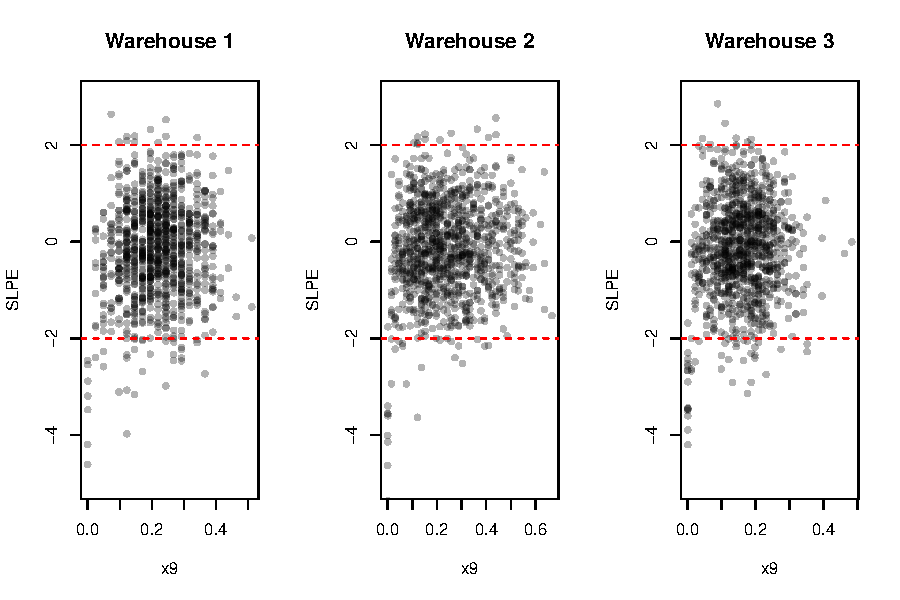
\includegraphics{fig-ds/first-resids.pdf}
 \caption{SLPEs plotted against $x_9$; the dashed red lines denote $\pm 2$ and the $x$ axis is on the standardised $[0,1]$ scale. We see, in each case, that there is a `tail' of residuals for small values of $x_9$. Each emulator has at least one SLPE larger than $4$ in modulus, suggesting a serious discrepancy between the emulator and $U(\bx)$. The vertical bands of residuals are present since $x_9$ takes values from a finite set. \label{Fig:first-loo}}
\end{figure}
To improve the emulator, we introduced a non-constant mean function: $\mu(\bx) = \beta_0 + \beta_1 \log (x_9 + 10^{-8})$. The addition of $10^{-8}$ avoids the undefined value $\log(0)$. The value $10^{-8}$ could be replaced by an unknown constant to be inferred, but we found that this initial guess value to satisfactory emulators. For the revised emulators, we integrated out the $\beta$ coefficients by adopting the prior specification $\beta_i \iid \mathcal{N}(0, 0.5^2)$ for $i \in \{0, 1\}$. This led to emulators with improved LOO diagnostics, which are illustrated in \cref{Fig:second-loo}. These residuals suggest that the revised emulator offers a better estimate of $U(\bx)$ than the first emulator. In this section we have only shown the SLPEs plotted against $x_9$; plots of SLPEs against inputs $x_1$ -- $x_{18}$ are given in \cref{App:resid2}.
\begin{figure}
 \centering
 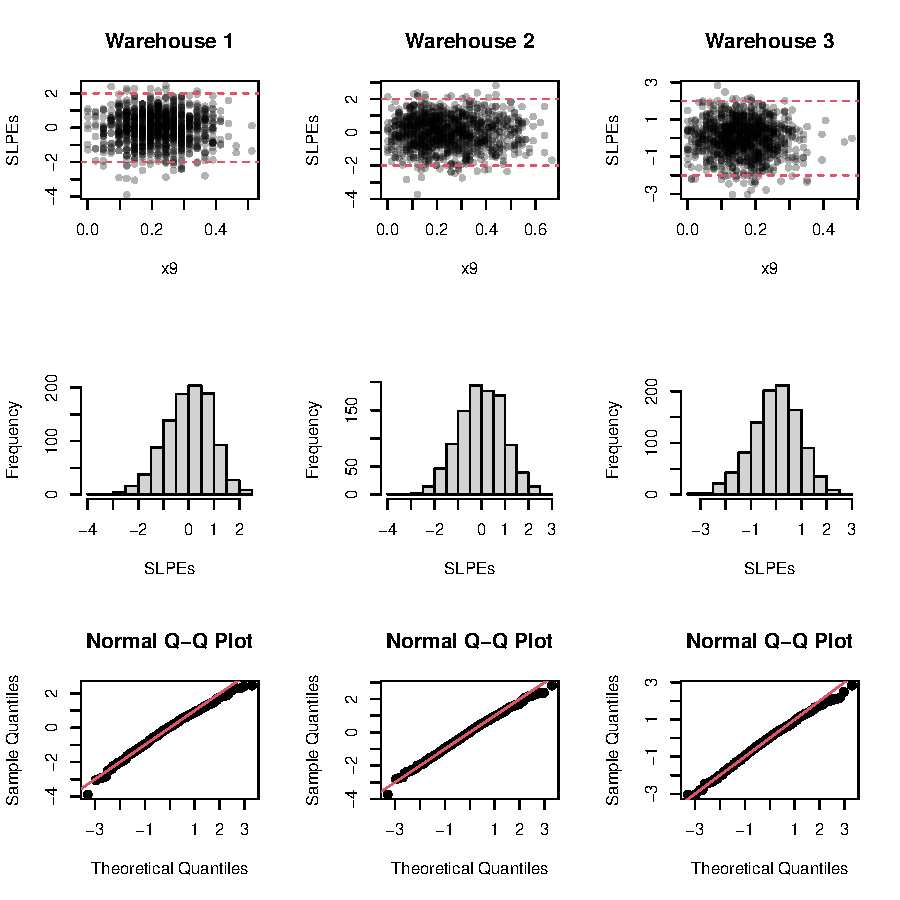
\includegraphics{fig-ds/second-resids.pdf}
 \caption{A suite of diagnostics based on SLPEs, organised in columns. Left column corresponds to Warehouse $1$, the middle column to Warehouse $2$ and the right column to Warehouse $3$. The top three plots show the SLPEs plotted against $x_9$ after incorporating the prior mean function $\mu(\bx) = \beta_0 + \beta_1 \log (x_9 + 10^{-8})$. Dashed red lines are at $\pm2$. The second row of plots are histograms of the SLPEs and the final row are Normal QQ plots, where the red line is the unit diagonal.\label{Fig:second-loo}}
\end{figure}
 A suite of diagnostic plots in \cref{Fig:second-loo} suggest that the emulator is an improved and appropriate surrogate for $U(\bx)$; the LOO residuals now appear to be uncorrelated with $x_9$, the histograms of the LOO errors are close to that of a standard Normal distribution (the distribution of SLPEs for Warehouse $1$ has a slightly longer left tail than one might expect) and the QQ plots further indicate the LOO errors are well described by a standard Normal distribution. We also verify that the cut off of $3$ is appropriate by checking quantiles of the Normal distribution. \cref{Tab:cred1} shows that over $95\%$ of the LOO errors lie in $(-3,3)$, thus there is agreement with Pukelsheim's $3\sigma$ rule and we are now in a position to rule out inappropriate decisions.
\begin{table}
 \centering
 \begin{tabular}{rrrr}
  \toprule
  Warehouse & SLPE Interval & Expected Proportion & Observed Proportion \\\cmidrule{1-4}
  $1$ & $(-2,2)$&$0.95$ & $0.968$\\
  &$(-3,3)$& $0.997$ & $0.998$ \\\cmidrule{1-4}
  $2$ & $(-2,2)$&$0.95$ & $0.967$\\
  &$(-3,3)$& $0.997$ & $0.999$ \\\cmidrule{1-4}
  $3$ &$(-2,2)$& $0.95$ & $0.964$\\
  &$(-3,3)$& $0.997$ & $0.998$ \\\bottomrule
 \end{tabular}
 \caption{Comparing the expected proportion to the observed proportion of SLPEs to lie within given intervals, assuming Normality of the SLPEs. The observed proportions are those from the improved emulator.}
 \label{Tab:cred1}
\end{table}
\subsection{Ruling out decisions}
Using the improved emulator, we can find the design point, $\hat{\bx}$, which maximises $\E\{U(\bx)\}$. In this case, $\hat{x}_{19} = 50$, so the decision belongs to Warehouse $1$. The other elements of $\hat{\bx}$ are given in \cref{Tab:optimiser}. Our uncertainty about $U(\hat{\bx})$ is characterised by
\begin{equation}
 U(\hat{\bx}) \sim \mathcal{N} (0.8314, 8.749 \times 10^{-5})
\end{equation}
\begin{table}
 \centering
 \begin{tabular}{lrrrrrrrrr}
  \toprule
  $i$ &1&2&3&4&5&6&7&8&9\\\cmidrule{1-10}
  $\hat{x}_i$& 1 & 4 & 9 & 7 & 2 & 4 & 9 & 1 & 13\\
  $\hat{x}_{i+9}$ &57.03 & 39.96 & 42.07 & 28.25 & 2.29 & 40.25 & 46.62 & 1.32 & 57.5\\
  \bottomrule
 \end{tabular}
 \caption{The estimated optimal decision reported on the decision scale rather than the $[0,1]$ scale. The warehouse is absent from the table and this decision corresponds to Warehouse $1$. The top row of variables corresponds to the number of spares of type $i$, the bottom row corresponds to the critical percentage for spares of type $i$. \label{Tab:optimiser}}
\end{table}
Now, Warehouse $1$ is in the NROY space as $I(\hat{\bx}) = 0$. We constructed a random, uniform sample of decisions ($N = 10^5$) within each warehouse and found that $90.87\%$ of decisions corresponding to Warehouse $1$ satisfied $I(\bx) < 3$ ($95\%$ CI: $(90.81, 90.93)\%$) whereas only $1.4 \times 10^{-3}\%$ of decisions corresponding to Warehouse $2$ are NROY ($95\%$ CI: $(6.52, 21.5)\times 10^{-3}\%$). Credible intervals were found using a Binomial model for the number of observed NROY decisions within Warehouse $i$, $M_i$, from a sample of $N_i$ random and uniformly distributed decisions. If the proportion of NROY decisions is $\alpha_i$ then \textit{a priori} $\alpha_i \sim Beta(a_i, b_i)$ and the sampling model for the number of NROY decisions observed from a random sample is $M_i \mid \alpha_i \sim Binomial(N_i = 10^5, \alpha_i)$. It is well known that the distribution of $\alpha_i \mid M_i$ is given by
\begin{align}
 \alpha_i \mid M_i &\sim Beta(A_i, B_i) \\
 A_i & = a_i + \sum_{j=1}^{N_i} \mathbb{I} ( I(\bx_{i,j}) \geq 3)\\
 B_i & = b_i + \sum_{j=1}^{N_i} \mathbb{I} ( I(\bx_{i,j} ) < 3)
\end{align}
where $\bx_{i,j}$ is the $j$th candidate decision for Warehouse $i$. For each warehouse, we took a flat prior for $\alpha$ ($a_i = b_i = 1$) and then the credible intervals are found as the $95\%$ highest posterior density intervals for $\alpha_i \mid M_i$.

Our random sample returned $0$ decisions in Warehouse $3$ that were NROY. To see if we could conclusively rule out Warehouse $3$ as a sub-optimal decision, we minimised the implausibility function for Warehouse $3$. To simplify the minimisation, we treated the discrete inputs as continuous. After running the optimiser $20$ times, our minimum implausibility was $\min I(\bx) = 7.36 > 3$. We are therefore satisfied that all decisions corresponding to Warehouse $3$ will be ruled out.

The nature of the NROY space for Warehouse $1$ is shown in \cref{Fig:wave1-w1-nroy}. We see that most decisions are green (NROY). The red, ruled-out decisions all seem to be those with very small values of $x_9$. For warehouse $2$, only $14$ out of $10^6$ points from the large random sample were retained as NROY. We have therefore presented only the NROY samples in \cref{Fig:wave1-w2-nroy}. For Warehouse $2$ we see that every $x_{10:18} < 0.5$ on the $(0,1)$ scale. This suggests a larger warehouse size affords us more time to buy in spares.
\begin{figure}
  \centering
  \includegraphics[width = 8in, angle=270]{fig-ds/wave1-wh1-landscape.pdf}
  \caption{A large uniform sample of decisions corresponding to Warehouse $1$. Green decisions are those that are NROY and red have been ruled out. Although $x_1$ was not explicitly included in the emulator, we have included it in this figure. Further note that the first $9$ inputs have been jittered with $\mathcal{N}(0, 9 \times 10^{-6})$ noise to aid visualisation. \label{Fig:wave1-w1-nroy}}
\end{figure}
\begin{figure}
  \centering
  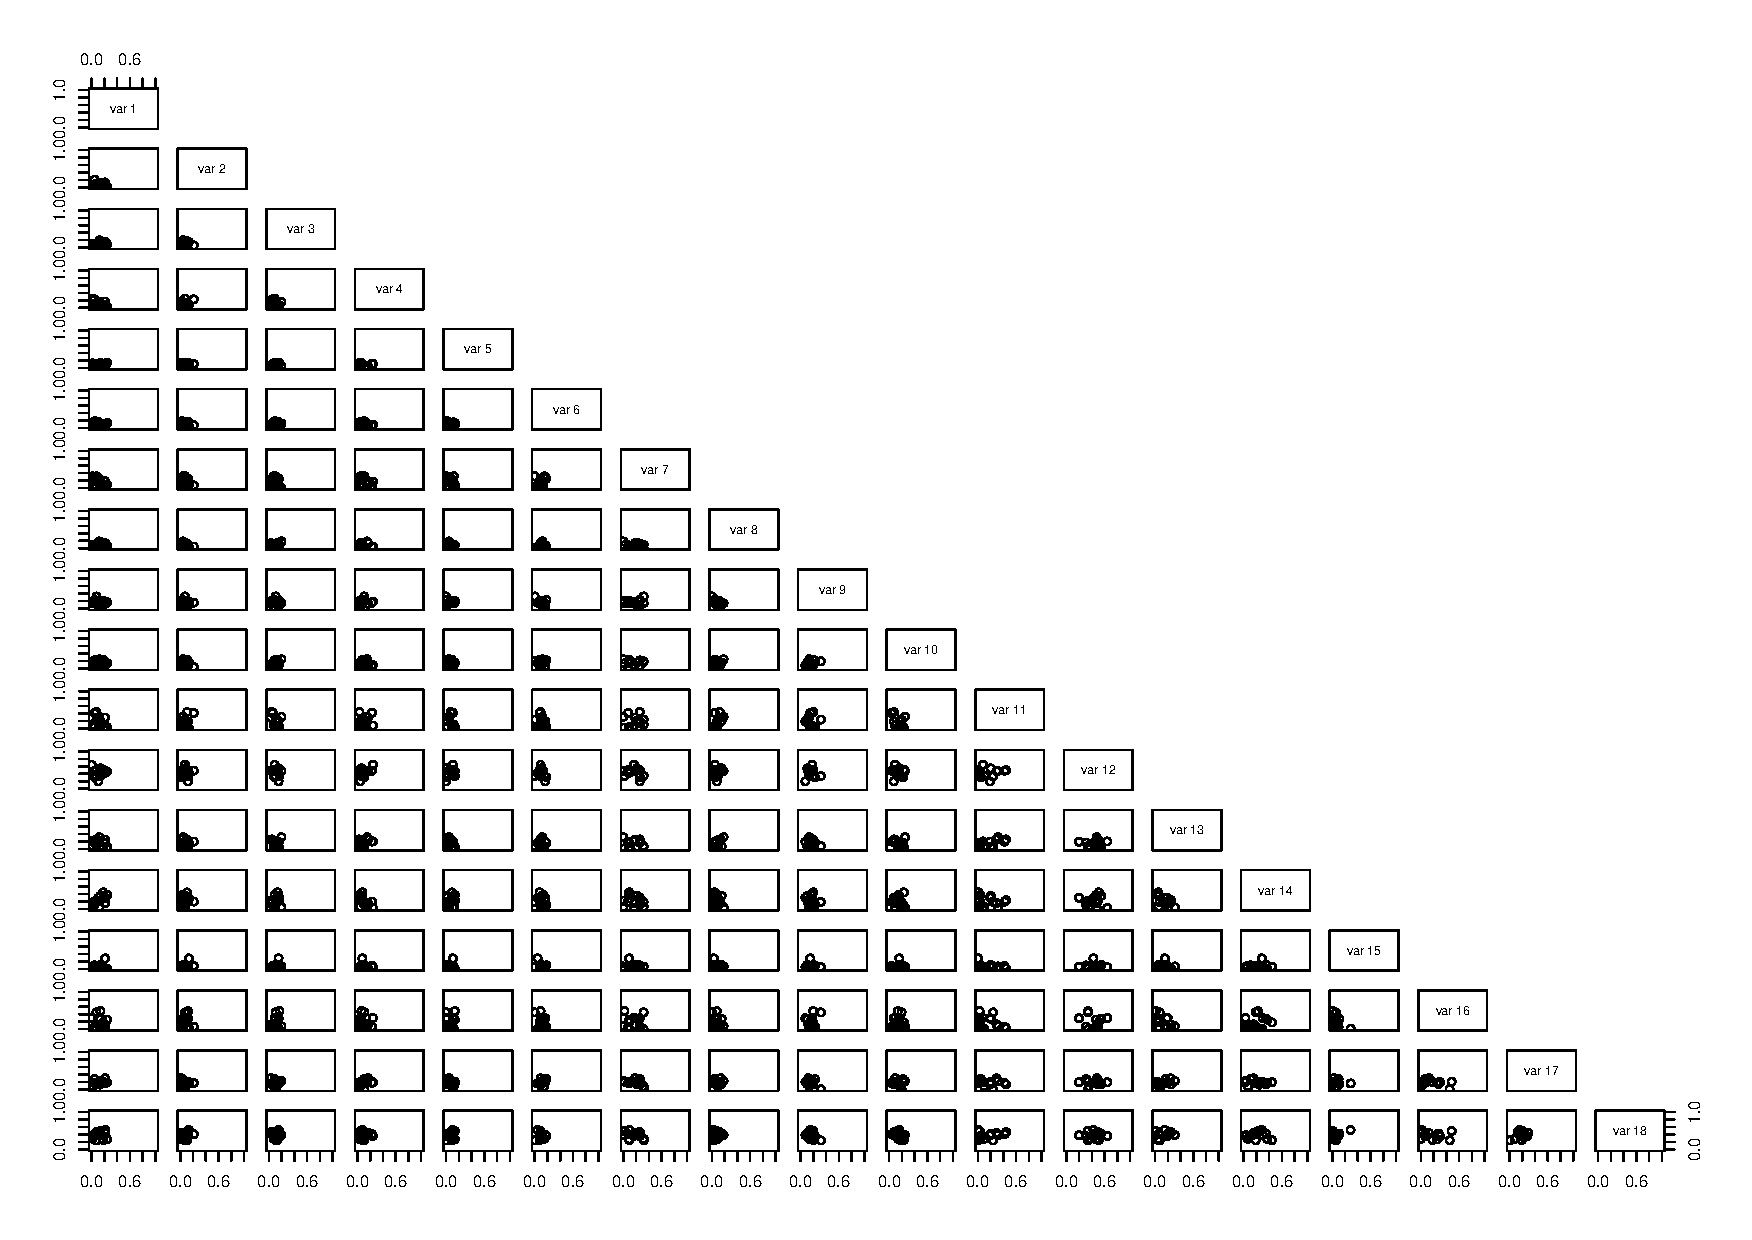
\includegraphics[width = 8in, angle=270]{fig-ds/wave1-wh2-landscape.pdf}
  \caption{A collection of NROY decisions corresponding to Warehouse $2$. Although $x_1$ was not explicitly included in the emulator, we have included it in this figure.\label{Fig:wave1-w2-nroy}}
\end{figure}

We have greatly simplified the analysis for the DM by applying a post-hoc history matching inspired idea to the BayesOpt routine to find decisions which are consistent with the approximate maximiser and find those which are clearly suboptimal. If desired, this would be a sensible place to stop the analysis and report our findings to the DM. However, the HM literature has shown that further probing can be advantageous \citep{Jackson2018, Vernon2022}.

\subsection{Constructing a wave $2$ design}

We follow the convention of further investigation within the NROY space to refine the set of sensible decisions. To do so, we need a design for a wave $2$ emulator. For Warehouse $1$, since the remaining NROY volume is quite large, simple rejection sampling will lead to a uniform design without much trouble. For Warehouse $2$, the NROY volume is a small fraction of the original volume, consequently, rejection sampling is inefficient.

To overcome the inefficiency of rejection sampling, we employ an adapted version of the slice sampler presented by \citet{Andrianakis2017a}. The adaptation addresses the discrete simplex aspect of the decision space and is presented in \cref{Alg:disc-slice}. The sum to unity constraint on the simplex means one decision variable is determined, given the rest. This algorithm does not include any continuous-valued components of $\bx$, however, since the algorithm is component-wise, we can first update the set of discrete components and then update the set of continuous components using \cref{alg:nroy-slice}.

\begin{algorithm}[h]
\caption{A single sweep of a component-wise slice sampler for generating NROY samples within the discrete simplex. \label{Alg:disc-slice}}
\begin{algorithmic}
\Require An indicator function $\mathbb{I}(\bx \in \calX_{k+1})$ for identifying inputs which are NROY, an initial NROY point $\bx_0 \in \calX_{k+1}$ where $\bx_0$ is an $m$ dimensional parameter vector. A set of $q+1$ unique, equally spaced, values $\mathcal{S} = \{ d_0, d_1, d_2, \ldots, d_{q-1}, d_q \}$ where $0 = d_0 < d_1 < \ldots < d_{q-1} < d_q = 1$.
\State $\bx^{*} \gets \bx_0$
\For{$i = 1$, $2$, $\ldots$, $m$}
 \State $I^{*} \gets 0$ \Comment{Initialise an indicator variable}
 \While{$I^* \neq 1$}
  \State Compute $d_p = 1 - \sum_{j \neq i} x^{*}_j$
  \State Draw $x_i \sim \mathcal{U} \{ d_0, d_1, d_2, \ldots, d_p \}$ \Comment{Change the $i$th input}
  \State $x^{*}_i \gets x_i$
  \State $x^{*}_1 \gets 1 - \sum_{j = 2}^m x_j^{*}$ \Comment{Force sum to unity constraint}
  \State $I^{*} \gets \mathbb{I}(\bx^{*} \in \calX_{k+1})$ \Comment{Evaluate the implausibility measure at the new input}
 \EndWhile
\EndFor
\State $\bx_1 \gets \bx^{*}$
\State Return $\bx_1$, the new NROY sample.
\end{algorithmic}
\end{algorithm}
\correction{As with \cref{alg:nroy-slice}, \cref{Alg:disc-slice} is not ergodic. However, as with \cref{alg:nroy-slice}, we can adapt \cref{Alg:disc-slice} to become ergodic in a similar way to \cref{alg:ergodic-slice}: we essentially re-run the algorithm from a collection of randomly chosen starting points. We write this out explicitly in \cref{alg:ergodic-disc-slice}.}

\begin{algorithm}[h]
\caption{An ergodic algorithm for simulating uniformly on of $\mathcal{S}^n_q \times [0, 1]^p$. \label{alg:ergodic-disc-slice}}
\begin{algorithmic}
\Require An indicator function $\mathbb{I}(\bx \in \calX_{k+1})$, a set of $q+1$ unique, equally spaced, values $\mathcal{S} = \{ d_0, d_1, d_2, \ldots, d_{q-1}, d_q \}$ where $0 = d_0 < d_1 < \ldots < d_{q-1} < d_q = 1$, the number of continuous inputs, $p$,  a number of replications, $R$, a required number of samples, $n =  n' \times R$, and a function $\texttt{slice\_sampler\_one\_step}(\mathbb{I}(\bx \in \calX_{k+1}), \bx_0)$ which takes an NROY point $ \bx_0 \in \calX_{k+1} \subseteq \mathcal{S}_q^n \times [0, 1]^p$, and returns a new NROY point.
\For{$r = 1, 2, \ldots, R$}
  \State {$I_r \gets 0$}
  \State Initialise a matrix $X_r$ with $m$ columns and $n'$ rows
  \While{$I_r \neq 1$}
    \State $\bx_{1, r} \gets \mathcal{U}(\mathcal{S}_q^n \times [0, 1]^p)$ \Comment{Simulate uniformly from the cross product of $\mathcal{S}^n_q$ and $[0, 1]^p$ }
    \State $I_r \gets \mathbb{I}(\bx{1, r} \in \calX_{k+1})$
  \EndWhile
  \For{$i = 2, 3, \ldots, n'$}
  \State $\bx_{i, r} \gets \texttt{slice\_sampler\_one\_step}(\mathbb{I}(\bx \in \calX_{k+1}), \bx_{i-1, r})$
\EndFor
\EndFor
\State Collect all $X_r$ into a single matrix $X$, with $m$ columns and $n$ rows.
\State Return $X$, the collection of uniformly distributed NROY samples.
%\Return $X$, a sample of $n$ NROy points.
\end{algorithmic}
\end{algorithm}

For low-dimensional, continuous-valued simplices, uniform sampling typically gives reasonable coverage of the margins. However, as the dimension increases, we encounter a problem. It becomes increasingly difficult for large values of $x_i$ to be sampled. Although we work with a discrete simplex, a continuous-valued simplex is easier to analyse and provides us with a good intuition for the marginal behaviour of a discrete simplex.

A uniform sample on the $k$ dimensional, continuous simplex is equivalent to sampling from a $Dirichlet(1_{k+1})$ distribution, where $1_{k+1}$ is a length $(k+1)$ vector of $1$s. A well known result states that if $\bm{X} \sim Dirichlet(\bm{\alpha})$ then the marginal distributions are given by $X_i \sim Beta(\alpha_i, \alpha_0 - \alpha_i)$ where $\alpha_0 = \sum_{j=1}^{k+1} \alpha_j$. Applying this result to the simplex means that a uniform sample on the $k$ dimensional simplex has $Beta(1, k)$ margins. Now for any $b \in (0,1)$, $\Pr (X_i > b) \to 0$ as $k \to \infty$. Although we have stated an asymptotic result, the effects are present even for moderate values of $k$. In \cref{Fig:beta-plot} we see plots of $\Pr (X_i > b)$ for various choices of $b$ over the range $k = 1, 2, \ldots, 13$. Note that we have $k = 8$ and thus $\Pr(X_i > 0.2) = 0.17$, $\Pr(X_i > 0.4) = 0.017$, $\Pr(X_i > 0.6) = 6.6 \times 10^{-4}$ and $\Pr(X_i > 0.8) = 2.6 \times 10^{-6}$. With emulators, we often have quite small samples sizes. Typically, designs have at most $1000$ points. From a decision support perspective, this is worrying. We want to consider a diverse set of decisions with a relatively small sample size. Therefore, we aim to construct a design which fills the space or, at least, targets areas of the decision space which are uncertain. This is especially important for Warehouse $1$ as the current NROY space is almost all of the Warehouse $1$ space.
\begin{figure}
 \centering
 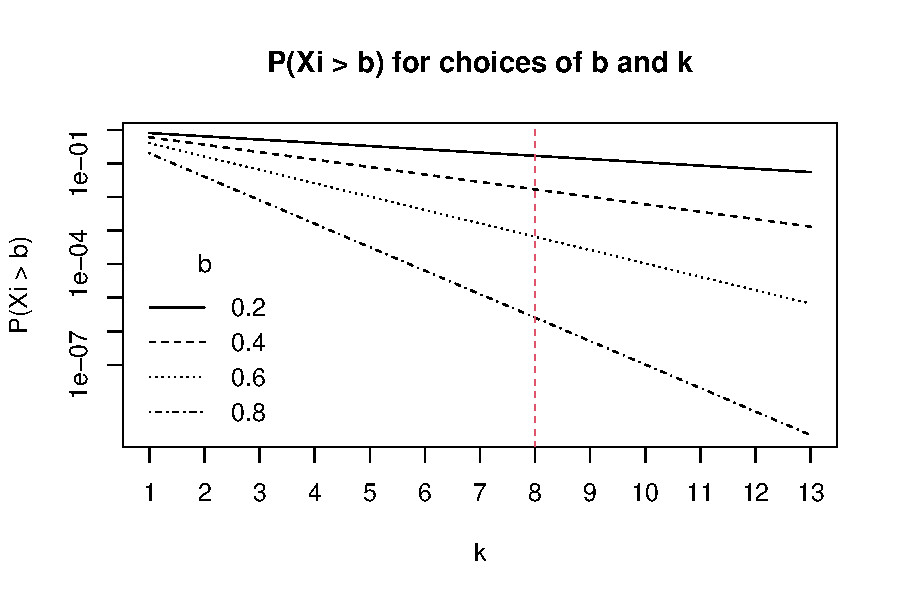
\includegraphics{fig-ds/beta-plot.pdf}
 \caption{Lines showing how $\Pr(X_i > b)$ decreases with $k$, the dimension of the simplex. The vertical, red dashed line corresponds to $k = 8$, the dimension of the simplex in our wind farm example. The black lines of various types correspond to different values of $b$. Note that the $y$ axis is on the logarithmic scale. \label{Fig:beta-plot}}
\end{figure}

One way to alleviate this problem is to force the design points to be far apart. This is a standard procedure. For example, maximin LHs achieve this goal by forcing the closest points to be as far away as possible, that is, maximising the minimum distance between design points. Our approach to `filling the space' will be to construct an approximate ALM (Active Learning McKay, \cref{Eq:std-alm}) design of size $n$. This exploits the fact that, in certain circumstances, posterior GP covariance matrices depend only on the locations of the design points and \textit{not} the response $y = f(\bx)$. The posterior design matrix will usually rely on parameters estimated from the data therefore there is some dependence on $y$. However, we can use estimated parameters from a previous experiment or specify the parameters. For a single warehouse, we proceed in the following way: first construct a large, uniform design within the NROY space of size $N>>n$. Call this design $\tilde{\calX}$. Next, using assumed GP hyperparameters (from the previous wave, for example), find the point $\bx^{(1)} \in \tilde{\calX}$ which maximises $\var\{ U(\bx) \}$. If a constant mean function is used, all points will have equal variance and so a random sample from $\tilde{\calX}$ can initialise the procedure. We then remove $\bx^{(1)}$ from $\tilde{\calX}$ and find the next point with largest variance, call this point $\bx^{(2)}$. We keep repeating this procedure until we have obtained $\bx^{(n)}$. Then the set $X = \{\bx^{(1)}, \bx^{(2)}, \ldots, \bx^{(n)}\}$ will be an approximate ALM design. Increasing $N$ will likely lead to a better approximation to an exact ALM design. Finding $\argmax_{\bx \in \tilde{\calX}} \var \{ U(\bx) \}$ is achieved by computing $\var \{ U(\bx) \}$ for all $\bx \in \tilde{\calX}$. This approach is useful in two ways. Firstly it allows us to construct a space-filling design, but it also allows us to perform post-processing of the slice sampler. Since the slice sampler is an MCMC method, the design is prone to auto-correlation. This post processing via ALM allows us to cope with a potentially autocorrelated MCMC chain. Rather than thinning the chain by a fixed factor (keeping every $t$-th iteration), we automatically choose points which are not close to each other.

We used this approach for both the remaining warehouses. The slice sampler was used to generate $N = 10^5$ candidate points for ALM designs of $n = 10^3$. For an ALM design, we first tried two different approaches. The first approach utilised our knowledge of $U(\bx)$ and used the GP hyperparameters of the emulator with mean function $h(\bx) = \beta_0 + \beta_1 \log (x_9 + 10^{-8})$. Since the emulator was fitted using an empirical Bayes approach, the posterior distribution of each $(\beta_0, \beta_1)$ pair is a direct consequence of the multivariate Normal equations. Therefore, we use the wave $1$ posterior for the $\beta$ parameters as the prior for the wave $2$ emulators. This means that our ALM acquisition function, for warehouse $i$, is
\begin{eqnarray}
 \alpha_i(\bx) = \sigma^{2}_{i} + h(\bx)B_ih(\bx)^T - K_i(\bx, X') \left\{K_i(X', X') + \lambda_i^2\right\}^{-1} K_i(X', \bx) \label{Eq:alm-nroy}
\end{eqnarray}
where $i \in \{1, 2\}$ denotes the choice of warehouse, $K_i(\bx, \bx') = h(\bx) B_i h(\bx)^T + C_i(\bx, \bx')$ is the GP covariance function for warehouse $i$ where $B_i = \var\{\beta^{(i)} \mid \mathcal{D}^{(i)} \}$, $\mathcal{D}^{(i)}$ is the set training data for warehouse $i$. $C_i(\bx, \bx')$ is the covariance function for the residuals from the mean function of warehouse $i$; we assume a squared exponential covariance function. As in \cref{Eq:alm-nroy}, $X'$ represents all locations already in the design. That is, points used to initialise the design as well as those that have been acquired. The second approach relied less on our knowledge of $U(\bx)$. The second design did not use knowledge of the mean function and thus the covariance function was simply a squared exponential. This is achieved by setting $B_i = 0$. We will call the first type of ALM design (with mean) ALMa, and the second (without mean) will be called ALMb. The hyperparameters of each squared exponential covariance function were taken from the wave $1$ emulators.

The ALM post-processing of each MCMC chain took approximately $4.5$ hours. This gave designs which led to $x_i$, for $i \in \{1, 2, \ldots, 9\}$, having wider margins than a random, uniform design of the same size. For this particular problem, the ALMa approach led to margins which were wider than uniform, as did the ALMb design.

The differences between the ALM designs and the uniform design for Warehouse $2$ are more subtle. We suspect this less dramatic difference is due to the fact that the NROY volume within the Warehouse $2$ space is a small subset of the original Warehouse $2$ space. \cref{Fig:alm-vs-unif2} shows that, again, the range of each margin for the ALM designs are typically wider than the uniform design. Some of the uniform margins are wider then the corresponding ALM margins, but those that are wider are only wider by a small amount. In both cases, the difference between the ALMa and uniform design for $x_9$ is very large. This is because we used a non-constant mean function which depends on $x_9$. In particular, the functional form $\beta_0 + \beta_1 \log (x_9 + 10^{-8})$ has large in magnitude values for small $x_9$. Since the variance is essentially the square of this, $\var\{\beta_0 + \beta_1 \log (x_9 + 10^{-8})\}$ is maximised when $x_9 = 0$.
\begin{table}
\centering
\begin{tabular}{rrr}
\toprule
  & \multicolumn{2}{c}{Warehouse} \\\cmidrule{2-3}
Design & $1$ & $2$ \\\cmidrule{1-3}
 ALMb & $0.72$ & $0.17$ \\
 Uniform & $0.35$ & $0.15$ \\\bottomrule
\end{tabular}
\caption{Values of $\min_{\bx, \bx' \in X} \rho (\bx, \bx')$, where $X$ is either the ALMb or the uniform (slice sampling) design. \label{Tab:min-distances}}
\end{table}

This led to the marginal density of $x_9$ having unsatisfactory properties. A comparison of the three designs is given in \cref{Fig:compare-x9}. This figure shows the marginal density of $x_9$ under three design schemes. ALMa, the ALM design which utilised knowledge of the mean function, is clearly not space-filling. For example, $985$ out of the $1000$ points are all exactly the same value, and there is a huge void from $0.2$--$0.8$. The uniform design gives a more diverse set of candidate decisions for us to query, but we see that the largest value of $x_9$ is $0.585$. ALMb provides a wide range of decisions (slightly narrower than ALMa) and lacks holes in the design. Since ALMb has a large range, but does not have any holes, we will use this design for our wave $2$ experiment. Maximising minimum distance is a common design heuristic. We computed the minimum distances, $\min_{\bx, \bx' \in X} \rho (\bx, \bx')$, where $\rho(\cdot, \cdot)$ is Euclidean distance, for the ALMb and uniform designs, which are given in \cref{Tab:min-distances}. We see that the minimum distances for the ALMb designs for warehouses $1$ and $2$ are larger than the minimum distances for the corresponding uniform designs, thus the ALMb designs improves a standard design heuristic. We also want to quantify how much larger, on average, the range of the ALMb design is than the uniform design. An appropriate metric here will the geometric mean of the relative widths of the margins of one design to the other:
\begin{equation}
 \delta_g (i) = \left( \prod_{j=2}^{18} \frac{\delta_{\text{ALMb},i,j}}{\delta_{\text{Uniform},i,j}} \right)^{\frac{1}{17}}
\end{equation}
where $\delta_{D, i, j}$ denotes the range of margin $j$ within warehouse $i$ for design type $D$. Our design has $17$ degrees of freedom and so we have removed the index $j=1$ from the product. Now we have $\delta_g(1) = 1.13$, which indicates, in a multiplicative sense, that the ALMb design has margins which are, on average $13\%$ wider than uniform. We also have $\delta_g(2) = 1.14$, so again, the ALMb design offers an improvement.

A similar effect is seen for $x_9$ within warehouse $2$. We see (\cref{Fig:compare-x9-2}) that, to a lesser extent than warehouse $1$, that the ALMa design has a large clump of points at the lower end of the range. The uniform and ALMb designs appear to be similar (apart from a small shift in location), perhaps this is because the NROY volume for warehouse $2$ is a fairly small fraction of the original space and thus, many extreme values may have been ruled out. Since we will be using the ALMb design, from hereon in we will refer to it as the ALM design.
\begin{figure}
 \centering
 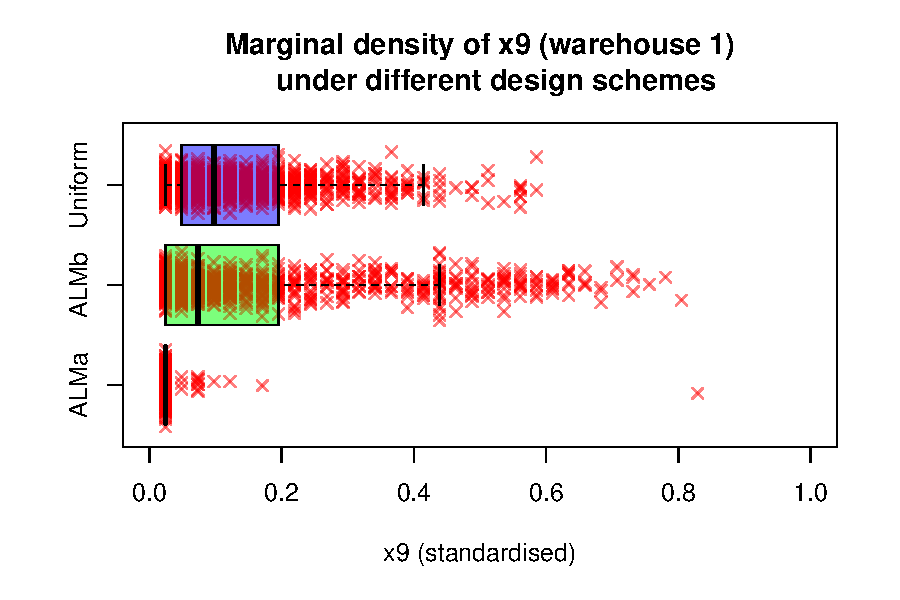
\includegraphics{fig-ds/compare-x9.pdf}
 \caption{Boxplots depicting the marginal density of $x_9$, for warehouse $1$, under three different design schemes. ALMa is the ALM design with the mean included, ALMb is the ALM design with no mean and Uniform is a uniform design generated by slice sampling. The red crosses denotes the values of $x_9$ from each design; these points are jittered vertically to aid visualisation. \label{Fig:compare-x9}}
\end{figure}
\begin{figure}
 \centering
 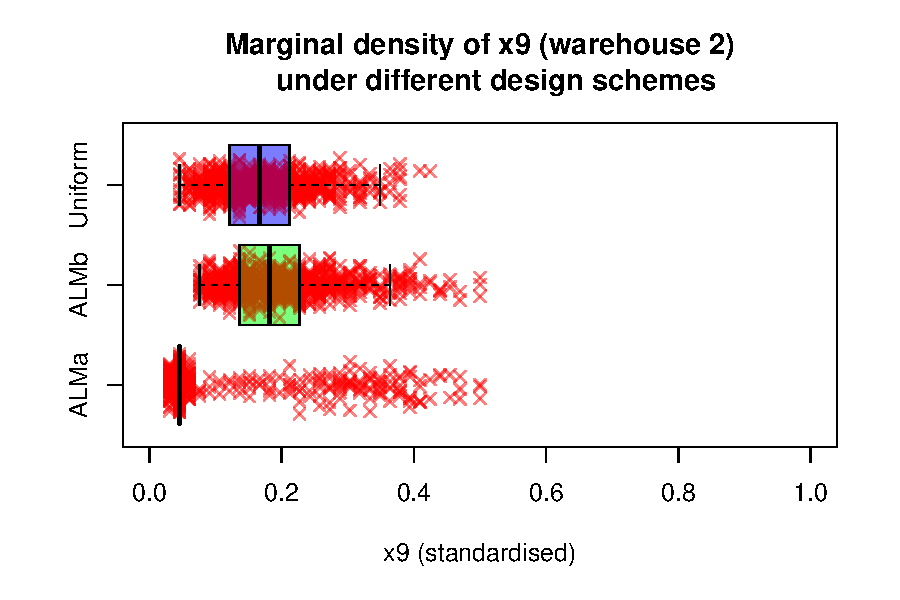
\includegraphics{fig-ds/compare-x9-w2.pdf}
 \caption{Boxplots depicting the marginal density of $x_9$, for warehouse $2$, under three different design schemes. ALMa is the ALM design with the mean included, ALMb is the ALM design with no mean and Uniform is a uniform design generated by slice sampling. The red crosses denotes the values of $x_9$ from each design; these points are jittered to aid visualisation. \label{Fig:compare-x9-2}}
\end{figure}
\begin{figure}
 \centering
 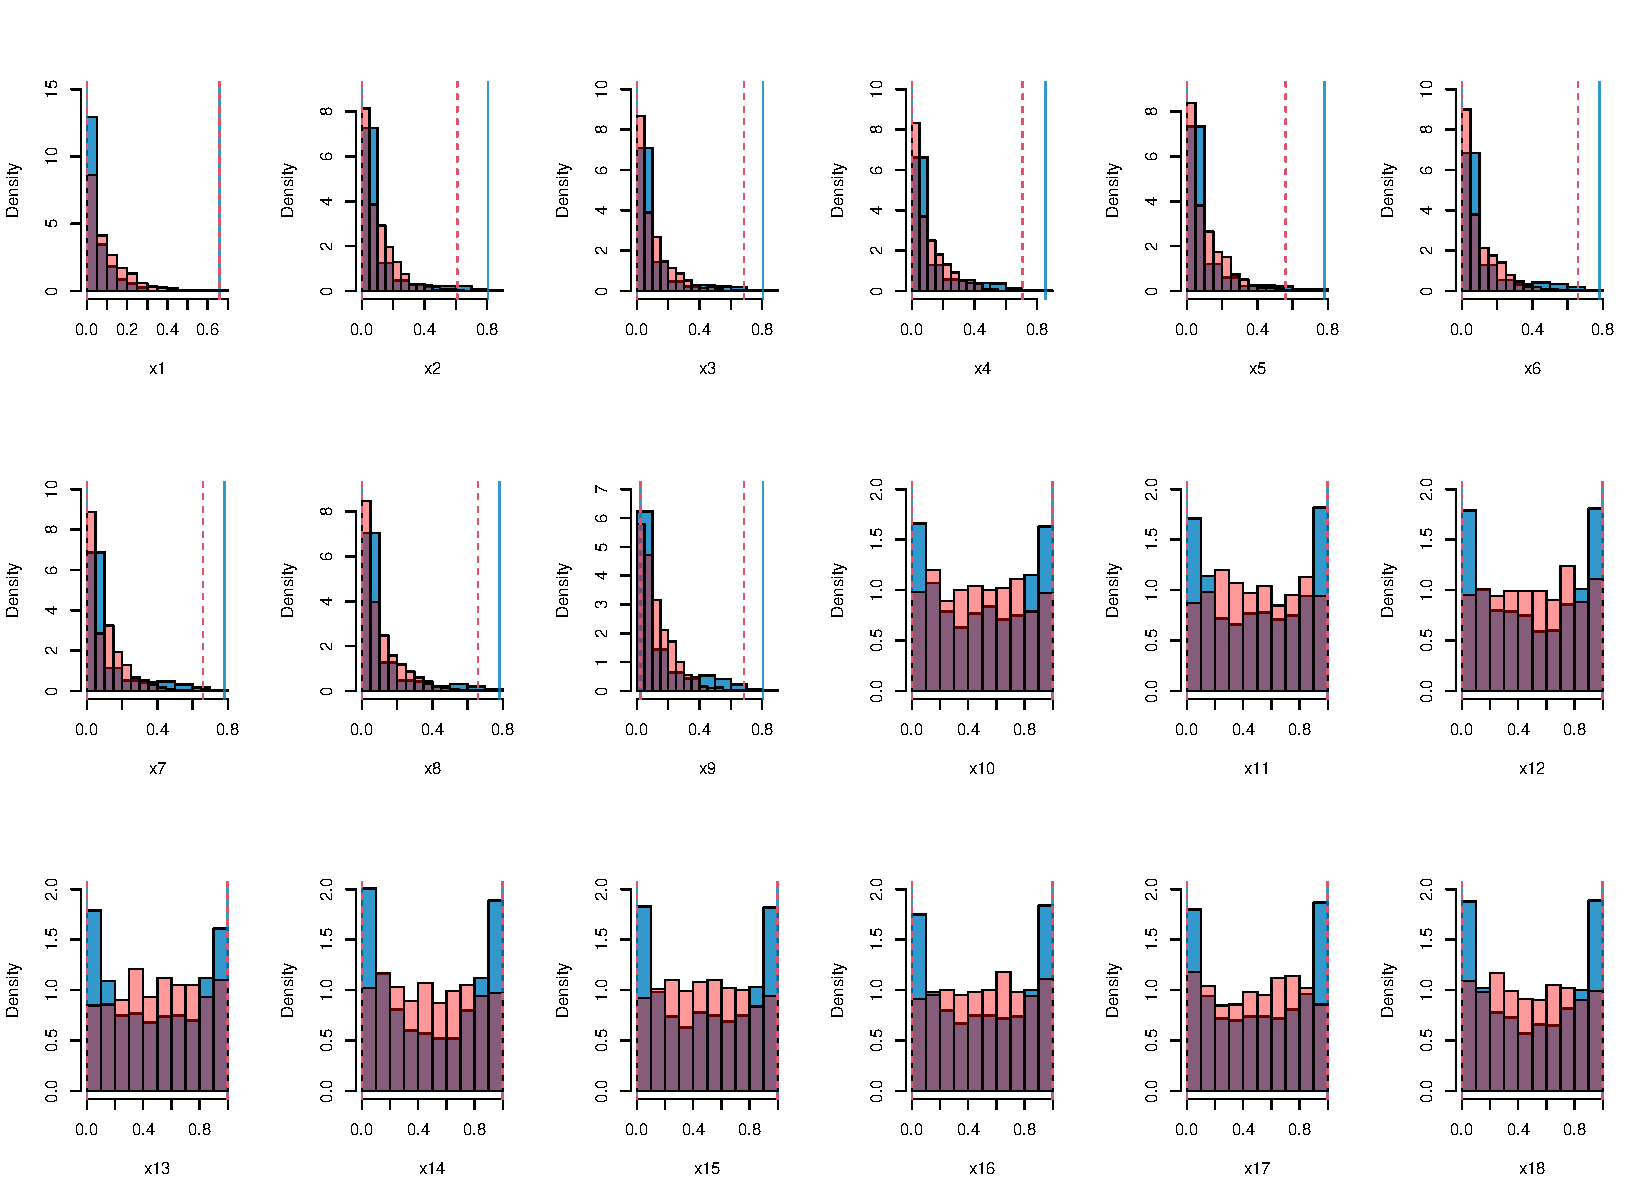
\includegraphics[width = 7.5in, angle = 90]{fig-ds/almnomean-vs-unif.pdf}
 \caption{Comparing the marginal behaviour of the ALM and the uniform designs for a sample size $n = 1000$ for Warehouse $1$. The ALM design is given as the blue histograms, whereas uniform are red. The limits of the ALM design are the solid blue lines, the dashed red lines are the limits of the uniform design.\label{Fig:alm-vs-unif}}
\end{figure}
\begin{figure}
 \centering
 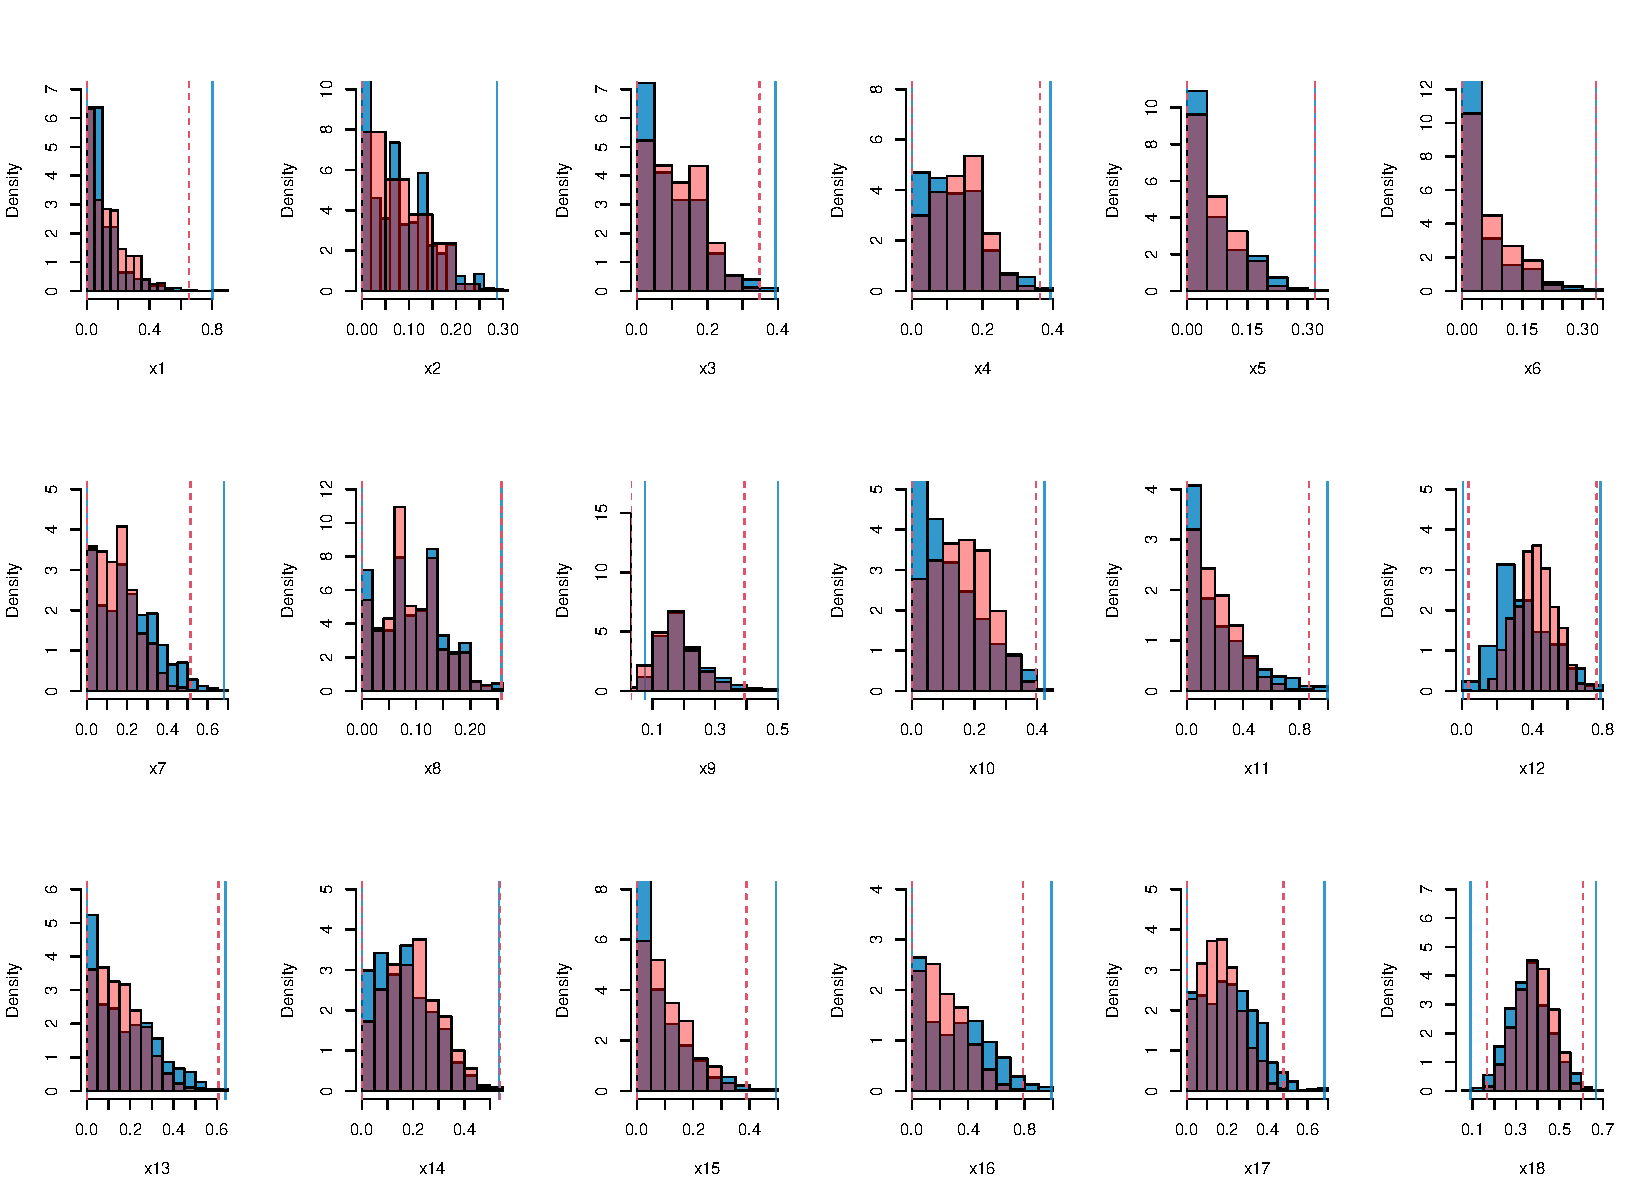
\includegraphics[width = 7.5in, angle = 90]{fig-ds/almnomean-vs-unif2.pdf}
 \caption{Comparing the marginal behaviour of the ALM and the uniform designs for a sample size $n = 1000$ for Warehouse $2$. The ALM design is given as the blue histograms, whereas uniform are red. The limits of the ALM design are the solid blue lines, the dashed red lines are the limits of the uniform design.\label{Fig:alm-vs-unif2}}
\end{figure}
\subsection{Wave $2$ emulators}

To construct the wave $2$ emulators we used the ALM designs discussed above. As with the wave $1$ emulators the training data is generated by averaging over $30$ realisations of $u(\bx)$ for each $\bx$.

For the GP hyperparameters, we adopted the same priors as the wave $1$ emulators, as these are relatively weak, but chosen to omit unrealistic values of the hyperparameters. We adopted the prior mean function $\mu(\bx) = \beta^{(i)}_0 + \beta^{(i)}_1 \log (x_9 + 10^{-8})$. The prior for each $\bm{\beta}^{(i)}$ was chosen as $\bm{\beta}^{(i)} \sim \pi(\bm{\beta} \mid \mathcal{D}^{(i)}, \Theta_i)$. That is, the posterior distributions from wave $1$ are adopted as wave $2$ prior distributions. We also tried including a more detailed mean function (and thus adjusted the prior on each $\beta^{(i)}$), however, we found that leave-one-out RMSE (\cref{Eq:rmse}) and Score (\cref{Eq:scoring-rule}) degraded when using a more detailed mean function. We therefore retain the functional form $\mu(\bx) = \beta^{(i)}_0 + \beta^{(i)}_1 \log (x_9 + 10^{-8}) $.
\begin{figure}
 \centering
 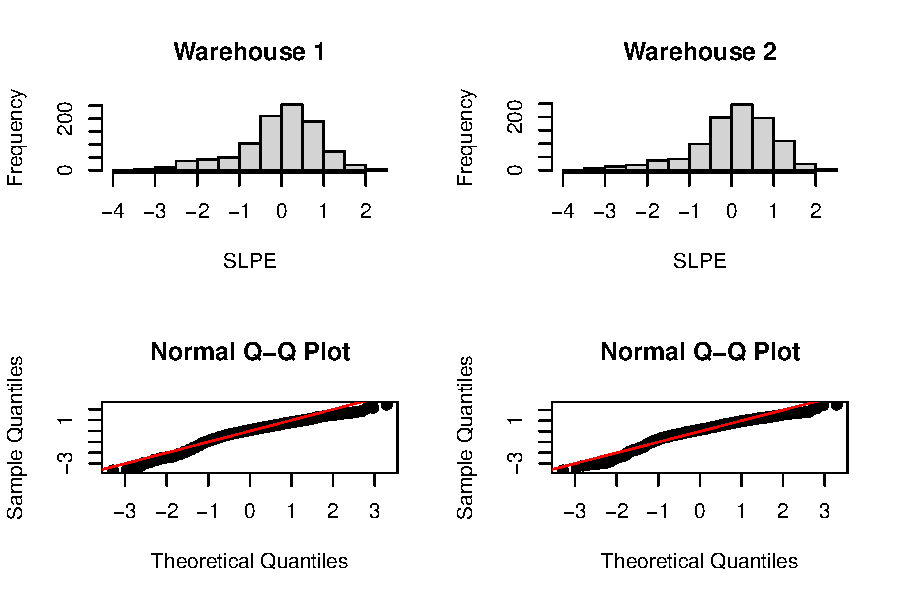
\includegraphics{fig-ds/diagnostics-wave2.pdf}
 \caption{Global diagnostics for the wave $2$ emulators. The left hand plots are for warehouse $1$ and the right hand for warehouse $2$. The top plots show histograms of LOO errors and the bottom plots are Normal QQ plots for the LOO errors.\label{Fig:w2-global-diag}}
\end{figure}
The emulators were fitted using our usual EB approach; assume a Normal likelihood, integrate out $\bm{\beta}^{(i)}$ and then finding a MAP estimate of the GP covariance structure. Global diagnostics are given in \cref{Fig:w2-global-diag}. We see there is some deviation from the Normality assumption. Namely, the left hand tail appears to be longer than the right hand tail. The excessive number of large, negative residuals implies there is some systematic under-prediction. This means the proportion of decisions ruled out may be larger than the proportion that would have been ruled out under a `perfect' emulator. When considering the problem of optimisation under uncertainty, we would argue this is preferable to the opposite scenario of many under-predictions with large error, since systematic under-prediction would lead to the NROY space being smaller than it should be. That is, we would be ruling out decisions that should be retained. Since this approach is conservative and aims to address uncertainty, we would rather retain some sub-optimal decisions (be inefficient) than rule out potentially good decisions (be ruthless). Plots of SLPEs against each inputs, for both warehouses, are given in \cref{App:resid3}.

However, the mean SLPE for warehouse $1$ is $-0.0452$ and the mean SLPE for warehouse $2$ is $0.00757$ which suggests that the SLPEs are not biased away from $0$. Moreover, we see that the observed proportions of SLPEs within $\pm2$ and $\pm3$ are close to their theoretical proportions, assuming Normality (\cref{Tab:cred2}). The observed proportions are slightly under the theoretical proportions, however, there is agreement with Pukelsheim's $3\sigma$ rule so we can perform another round of iterative refocussing with confidence in the calibration of the approach.
\begin{table}
 \centering
 \begin{tabular}{rrrr}
  \toprule
  Warehouse & SLPE Interval & Expected Proportion & Observed Proportion \\\cmidrule{1-4}
  $1$ & $(-2,2)$&$0.95$ & $0.944$\\
  &$(-3,3)$& $0.997$ & $0.995$ \\\cmidrule{1-4}
  $2$ & $(-2,2)$&$0.95$ & $0.954$\\
  &$(-3,3)$& $0.997$ & $0.992$ \\\bottomrule
 \end{tabular}
 \caption{Comparing the expected proportion to the observed proportion of SLPEs to lie within given intervals, assuming Normality of the SLPEs for the wave $2$ emulators.}
 \label{Tab:cred2}
\end{table}
\subsection{What is the maximiser?}
Although our philosophy towards decision making views the problem as having a set of sensible solutions, rather than one optimal solution, the HM inspired approach still needs a `best' value to rule out decisions. If our simulator was deterministic, we would simply take the largest value seen so far. However, we are working with a stochastic simulator. The uncertainty about the largest expected utility is an additional complication.

After the first wave, taking the largest expected utility, amongst the design points, is a natural choice for `best'. However, the wave $2$ emulators offer a new perspective of $U(\bx)$. The purpose of the wave $2$ emulator is to explore a diverse set of decisions (via an ALM design) rather than to exploit knowledge of $U(\bx)$ to optimise it. Since the wave $2$ emulator was not designed to optimise $U(\bx)$, should we trust its maximiser?

If we plug $\hat{\bx}_1$ into the wave $2$ emulator, we obtain $U(\hat{\bx}_1) \sim \mathcal{N}(0.790, 2.54\times10^{-4})$ which is rather different from the wave $1$ prediction. This is troublesome as it is not clear how to define our implausibility measure, which is reliant on the distribution of $U(\bx)$, and how it is correlated with $U(\bx')$. However, $\tfrac{|0.790 - 0.831|}{\sqrt{2.54\times10^{-4} + 8.75\times 10^{-5}}} = 2.22 < 3$ so these two characterisations of uncertainty about $U(\hat{\bx}_1)$ are in some sense compatible with each other. If we search the wave $2$ design, the largest expected utility belongs to warehouse $1$ and is characterised by
\begin{equation}
 U(\hat{\bx}_2) \sim \mathcal{N}(0.818, 2.47 \times 10^{-4}).
\end{equation}
Now, $\E \{ U(\hat{\bx}_2) \}$ is much closer to $\E\{U(\hat{\bx}_1)\}$; note that $|\tfrac{(0.831 - 0.818)}{\sqrt{8.75 \times 10^{-5} + 2.47 \times 10^{-4}}} | = 0.725$, thus relative to their uncertainties, these two characterisations of the optimum value are fairly close.
One solution to this problem is to perform sensitivity analysis: perform the analysis for both potential maximisers and see how different the results are. To perform the sensitivity analysis we will use $\hat{\bx}_1$ and take our uncertainty about $\hat{\bx}_1$ as characterised by the wave $1$ emulator. Our uncertainty about $\hat{\bx}_2$ will be characterised by the wave $2$ emulator.

This means there will be two possible implausibility measures. They are, for $\bx \in \calX_2$
\begin{align}
 I_{2,1}(\bx) &= \frac{\E^{(1)}\{U(\hat{\bx}_1)\} - \E^{(2)} \{U(\bx)\} }{\sqrt{\var^{(1)} \{U(\hat{\bx}) \} + \var^{(2)}\{U(\bx)\} }}\\
 I_{2,2}(\bx) &= \frac{\E^{(2)}\{U(\hat{\bx}_2)\} - \E^{(2)} \{U(\bx)\} }{\sqrt{\var^{(2)} \{U(\hat{\bx}) - U(\bx)\} }}
\end{align}
where the $(j)$ superscript denotes the expectation/variance at the $j$th wave of emulation. The $i,j$ subscript denotes that this is the implausibility at wave $i$ and we are using $\hat{\bx}_j$ as the `reference' value for HM.

\subsection{Second round of refocussing}
\begin{table}
	\centering
	\begin{tabular}{llrr}
		\toprule
  Wave & Best value & \multicolumn{2}{c}{Warehouse} \\\cmidrule{1-4}
  Wave $2$ only& & $1$ & $2$ \\
  &$\hat{\bx}_1$ & $50.5\%$ & $99\%$ \\
  &$\hat{\bx}_2$ & $90.8\%$ & $100\%$\\\cmidrule{1-4}
  Both waves& & $1$ & $2$ \\
  &$\hat{\bx}_1$ & $45.89\%$ & $1.39\times10^{-3}\%$ \\
  &$\hat{\bx}_2$ & $82.51\%$ & $1.40\times10^{-3}\%$ \\\bottomrule
	\end{tabular}
	\caption{Estimated proportion of the decision space remaining for each warehouse. The top half of the table is the reduction in space due to the wave $2$ emulators, having already reduced the space by wave $1$ emulators; the bottom half is the total reduction in NROY space from both waves of emulation. \label{Tab:compare-nroy}}
\end{table}
To assess the reduction in the NROY space we first use $I_{2,1}(\bx)$ as an implausibility measure. We will then use $I_{2,2}(\bx)$. Both measures will use the cut off of $3$ to determine which points have been ruled out. To estimate the reduction in the NROY space (compared to the previous wave) we will use a random, uniform sample of $1000$ points which were deemed not implausible after the first wave of emulation. The reduction in NROY space for each warehouse, using the different implausibility measures, is given in \cref{Tab:compare-nroy}. Using $\hat{\bx}_2$ as the maximiser leaves the NROY space essentially unchanged; it offers no reduction whatsoever in the space of warehouse $2$ and removes under $10\%$ of the space for warehouse $1$. When using $\hat{\bx}_1$ as the maximiser, we obtain a modest reduction in NROY space for warehouse $1$ and a small reduction in the space for warehouse $2$.

We will use $\hat{\bx}_2$ as the maximiser since it represents our current understanding of $U(\bx)$. This does not reduce the NROY space, which is somewhat frustrating. However, we should not to rule out decisions solely for the sake of ruling out decisions. This poses a question; since $\E\{U(\hat{\bx})\}$ has decreased, and $\var\{U(\hat{\bx})\}$ has increased, should we go back a wave and re-introduce decisions that were ruled out? We will not do this, but, \citet{baker-thesis2021} considers the notion of a flexible NROY space and shows that allowing the NROY region to shrink as well as grow protects against flaws in emulators from early waves. \citet{baker-thesis2021} shows, for a small set of simple examples, that the flexible approach can be advantageous in finding the `correct' NROY space.
\subsection{Termination of iterative refocussing}
After performing these two waves of analysis, we have used, approximately, a total of $22 \text{ cores} \times 5 \text{ training rounds} \times 6 \text{ days } \approx 1.8 \text{ years}$ of CPU time on generating training data for the emulators. This is based on the assumption that running Athena at $1000$ inputs, each replicated $30$ times, will take $6$ days (over $22$ cores). Training runs of Athena for this analysis took in the region of $5$-$7$ days, therefore $6$ days is a reasonable approximation. There is also the issue of queuing on HPC facilities which can be of the order of several days during busy periods. In terms of wall-clock time, we used a total of around $14$ days computing time. Another round of emulation would take approximately another $6$ days in training time. None of our calculations have included the human time required to perform analyses, the computational cost of fitting and validating of emulators or the computational cost of a design. For this reason, combined with the very small reduction in the NROY space we now terminate our iterative procedure.

Since we have terminated our procedure, we can calculate what proportion of decisions are NROY compared to the original set. This quantity is given by
\begin{align*}
 |\calX_{\text{NROY}}| &= \frac{0.8251 \times {49 \choose 8} + 1.39 \times 10^{-6} \times {74 \choose 8} + 0 \times {99 \choose 8}}{{49 \choose 8} + {74 \choose 8} + {99 \choose 8}}\\
 &= \frac{3.72 \times 10^8}{1.87 \times 10^{11}}\\
 &= 1.99 \times 10^{-3}
\end{align*}
which is a reasonable reduction in the size of the NROY volume; around $0.2\%$ of the original decisions have been deemed NROY. Note that we have completely ruled out warehouse $3$, and the number of decisions remaining from warehouse $2$ is tiny. Most of our remaining decisions correspond to warehouse $1$. By ruling out many decisions, we have greatly simplified the problem for the DM.
\section{Incorporating the DM: evaluating the consequences of decisions}
The final aspect of our analysis contains two parts. First we will provide the DM with a small set of NROY decisions. Displaying the consequences of a large set may overwhelm the DM and thus they may not be able to adequately assess the relative merits of each decision. These are decisions which are not clearly worse than $\hat{\bx}_2$. For each decision put forward to the DM, we will present the decision alongside the consequences of that decision. Recall, the consequences are the choice of warehouse, the availability time series and the restoration policy. We will present many replicates of the availability times series to the DM to communicate that this is an uncertain consequence.

The DM then has two tasks. The first task is to provide feedback on the decision space. If the DM finds believes that the given decisions are not consistent with their preferences, we must go back to the start of our analysis and perform the entire task again; re-elicit attributes, consequences, the functional form and parameters of the utility function \citep{Smith2010}. However, this is very computationally expensive so, if the DM does reject all of the decisions shown, we could first present a new sample of decisions. Note that this step is computationally expensive because one consequence relies on running the Athena simulator. However around $30$ replicates for a small handful of decisions can be computed in about an hour on the Rocket HPC facility, or overnight on a modern desktop computer. If the DM is not satisfied, it may be worth trying to optimise a single consequence. For example, if the DM was not happy with the availability trajectories we have produced from the NROY space, it would be worth investigating if there are \textit{any} availability trajectories within the initial decision space that the DM is happy with. We should also remind ourselves that decision analysis allows us to make the best decision, however, it is entirely possible that there are no `good' decisions, but rather, we must find the least worst option. For example, suppose you must make a long journey. You can either take the train, which takes $12$ hours and involves multiple connections, or you can take a $1$ hour flight. Further suppose you are environmentally conscious, and are aware that taking a flight is much more harmful to the environment than the train. Both decisions have obvious disadvantages and you might be unhappy with both prospects, but there will still be an optimal decision.

If the DM finds one or more solutions satisfactory, they must then decide which decision to make. This decision should solely be that of the DM.
\subsection{Presenting NROY decisions to the DM}
Since no real DM is involved in the analysis, we chose a set of $12$ decisions to present to our fictitious DM; $6$ from each warehouse. One was chosen as $\hat{\bx}_2$, another was chosen as the decision which maximised the wave $2$, warehouse $2$ emulator and a further $5$ random decisions from each warehouse within the NROY set. The values of $x_{1}$ -- $x_{18}$ for each of these decisions is given in \cref{Tab:final-dec}. The first $6$ decisions corresponds to warehouse $1$ decisions, the final $6$ to warehouse $2$. The $6$th decision is $\hat{\bx}_2$ and the $12$th decision is the decision which maximised the wave $2$, warehouse $2$ emulator. If a DM were to be involved, they may request the analyst to further investigate particular decisions, provided they are NROY.

We ran the Athena simulator $300$ times at each of these input configurations to give the DM a detailed picture of the availability trajectories one could see if we made any of these $12$ decisions. Allowing the DM to choose one of these decisions for themselves has the advantage of allowing the DM to bring in any additional information that was not given to the analyst. This ensures that the DM's preferences are honoured if the elicited utility function is a misrepresentation of their beliefs.
\begin{figure}
 \centering
 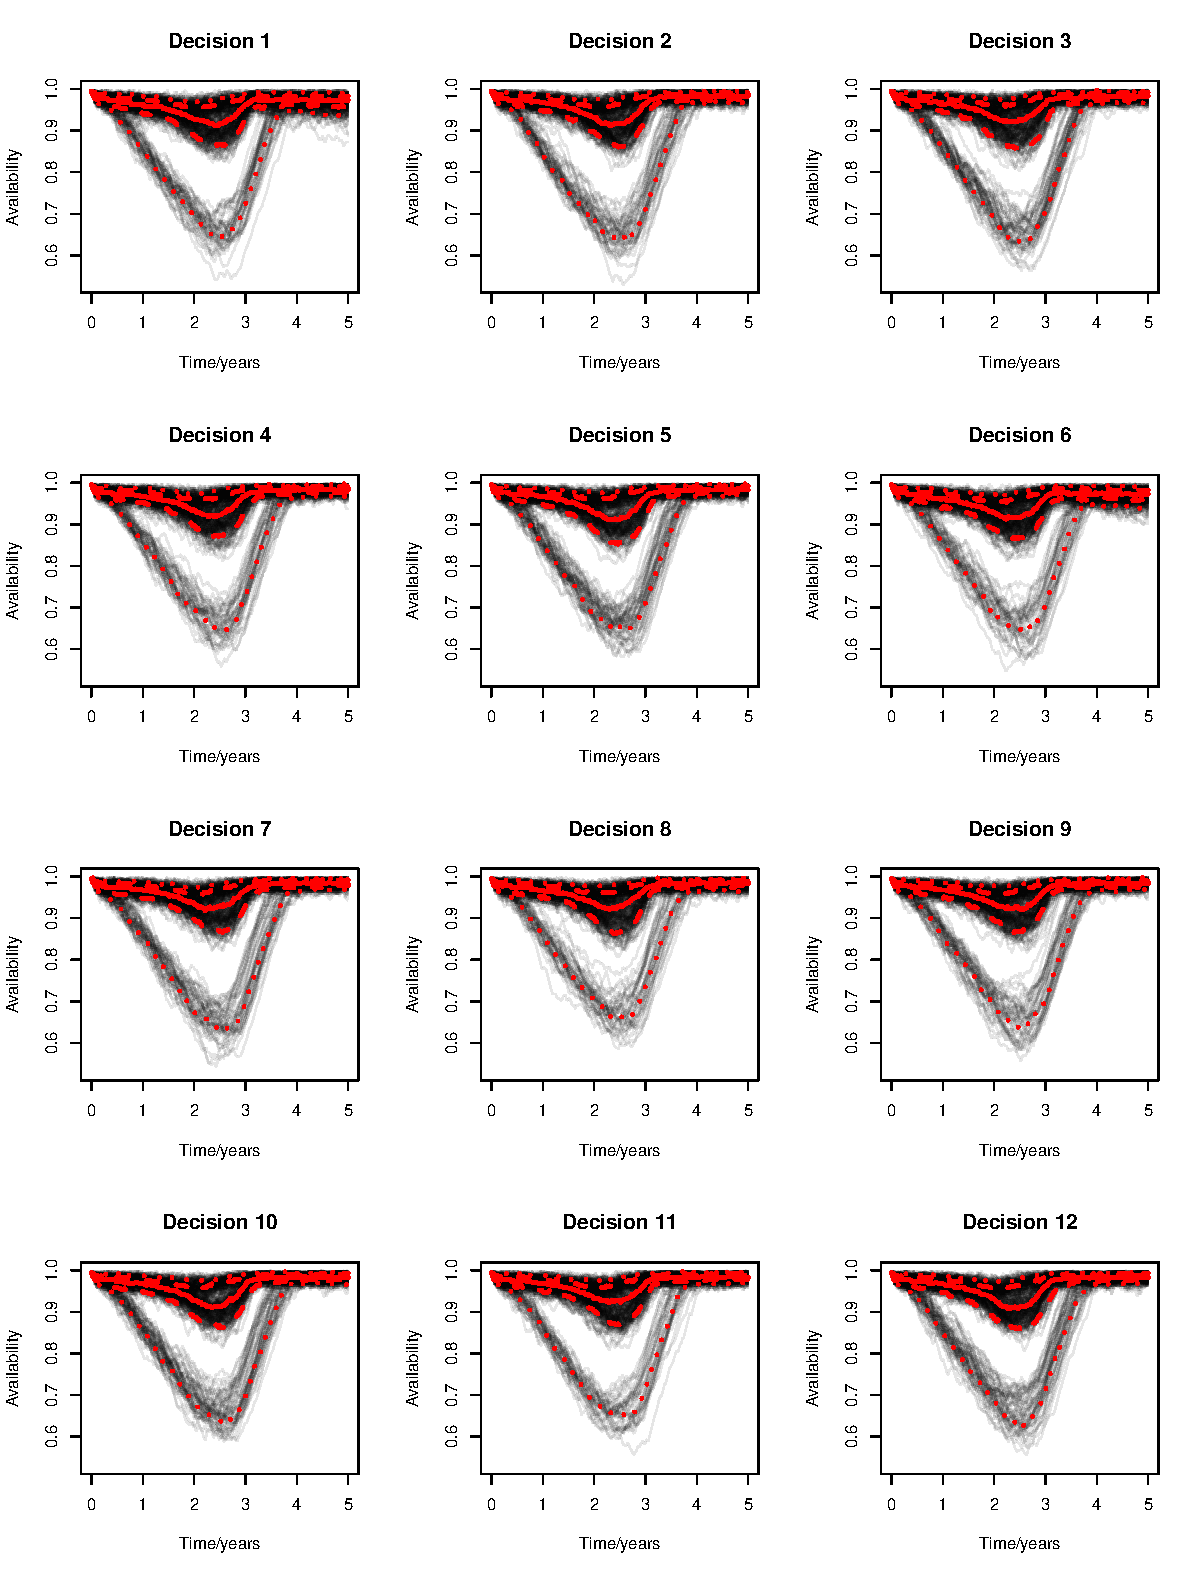
\includegraphics[width=\textwidth]{fig-ds/final-decisions-bold.pdf}
 \caption{Each sub-figure shows $300$ availability trajectories (grey lines) for each of the decisions given in \cref{Tab:consequences}. The solid red line represents the median availability trajectory for a decision, the dashed red lines correspond to $20\%$ and $80\%$ quantiles for the availability and the dotted red lines represent $5\%$ and $95\%$ quantiles for the availability. Quantiles are all point-wise.\label{Fig:final-avail}}
\end{figure}
\begin{sidewaystable}
\centering
\pgfplotstabletypeset[
multicolumn names,
col sep = comma ,
string type ,
every head row/.style ={ %
before row ={ %
\toprule
& \multicolumn{18}{c}{Decision variable ($x_i$)}\\
\cmidrule{2-19}\\
} ,
after row ={\midrule}
} ,
every last row/.style={after row =\bottomrule}
] %
{code-for-plots/sensible-decisions2.csv}
\caption{The values of $x_1$--$x_{18}$ for each of the $12$ decisions presented to the DM. Note that the first $6$ decisions correspond to warehouse $1$ ($x_{19} = 50$) and the final $6$ corresponds to warehouse $2$ ($x_{19} = 75$).\label{Tab:final-dec}}
\end{sidewaystable}
In \cref{Fig:final-avail} we see that the distribution of availability trajectories is very similar for the $12$ examples. By eye, it is essentially impossible to tell them apart. Each set of trajectories seems to have two modes. The `main' mode has the availability trajectories typically sitting in the region of $[0.9,1]$ for all $\text{Time} \in [0,5] \text{ years}$. The `minor' mode has a prominent dip in availability in for when Time is in the region of $[2,3]$ years; the availability drops to a minimum which is typically in the range $[0.6, 0.7]$.
\subsection{Retrospective validation of assumptions}
We now wish to (retrospectively) verify three aspects of our analysis. Our maximin design was constructed from, essentially, one long run of \cref{alg:nroy-disc}, rather than the ergodic variant --- we need to check that the Markov chain is irreducible (that is, not ergodic). Next, we relied on Pukelsheim's $3\sigma$ rule to determine which decisions are (not) consistent with the (estimated) optimal decision. We can only use Pukelsheim's $3\sigma$ rule when $U(\bx)$ has a continuous, unimodal distribution; we should verify this assumption. Finally, we should check that decisions from the final NROY set are indeed consistent with our findings.

\subsubsection{Checking the Markov Chain is irreducible}

To verify that the Markov chain used to generate a large candidate design is indeed irreducible, we implement \cref{alg:ergodic-disc-slice} with $R=30$ repeated runs, $n' = 1000$ within-chain runs for a total sample size of $N = 30000$. This is performed for each of warehouses 1 and 2.

To investigate as to whether or not the chain is reducible, we first performed principal components analysis to obtain a low-dimensional visualisation of the NROY samples. The first two principal components are shown for the two samples of $N = 30000$ NROY points generated from \cref{alg:ergodic-disc-slice} are shown in \cref{Fig:check-ergodic}.

\begin{figure}
  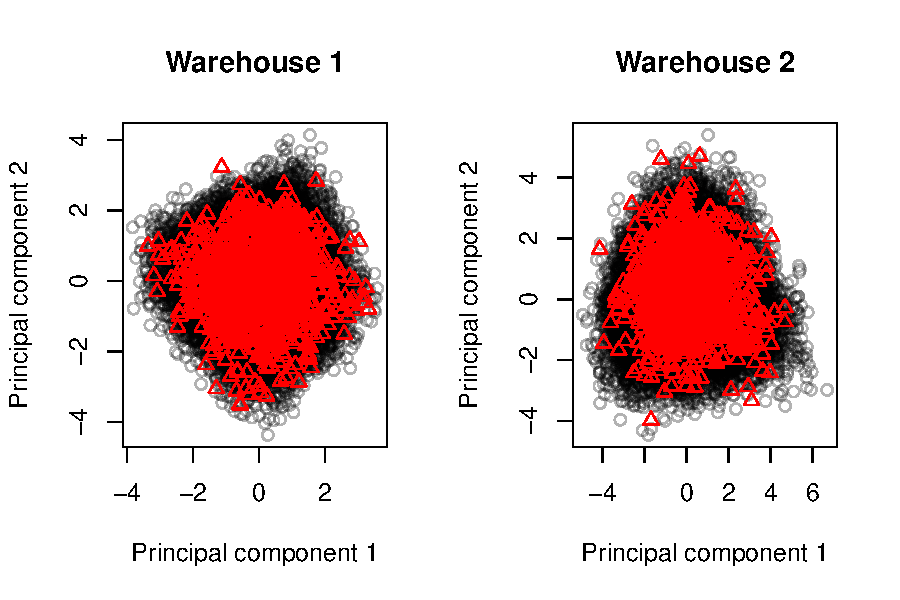
\includegraphics[width = \textwidth]{fig-ds/check-ergodic.pdf}
  \caption{For each warehouse, the figures show the first two principal components of a large collection of uniform NROY samples. The black circles are points from all chains, whereas the red triangles are a all the points from just one of the parallel runs. We see in both cases, that there is no evidence of a disconnected NROY region.\label{Fig:check-ergodic}}
\end{figure}

In each of the subfigures of \cref{Fig:check-ergodic}, there is no evidence to suggest that the NROY region is a union of disconnected regions. The red triangles --- the points from just one of the parallel runs --- have a similar joint distribution to all other samples. Further, the samples all appear to come from one connected region, rather than two or more disconnected sub-regions. Note that these samples are uniform across the NROY region and not processed to form (e.g.) a maximin design.

\subsubsection{Pukelsheim's $3\sigma$ rule}
Our history matching procedure has relied on Pukelsheim's 3$\sigma$ rule which states that $P(|U(\bx) - \mu| > 3\sigma) < 0.05$ under two assumptions. Firstly, $U(\bx)$ must be continuous. This is satisfied as $u(\bx)$ is a smooth function of $\bx$ and availability is a continuous-valued random quantity. The second assumption is that $U(\bx)$ must be unimodal. The sub-figures within \cref{Fig:final-avail} all show that the availability distribution has at least two modes. By the CLT, we would expect our training outputs, $y(\bx)$, to be approximately Normal (and thus unimodal) as they are constructed via sample means. However, it is important to remember that the CLT is only an asymptotic result and offers no general guarantee for samples sizes $n < \infty$. To verify that the training data are unimodal quantities, we perform a simple bootstrap procedure to estimate the sampling distribution of $y(\bx) = (1/30) \sum_{i=1}^{30} u(\bx)_i$.
\begin{figure}
 \centering
 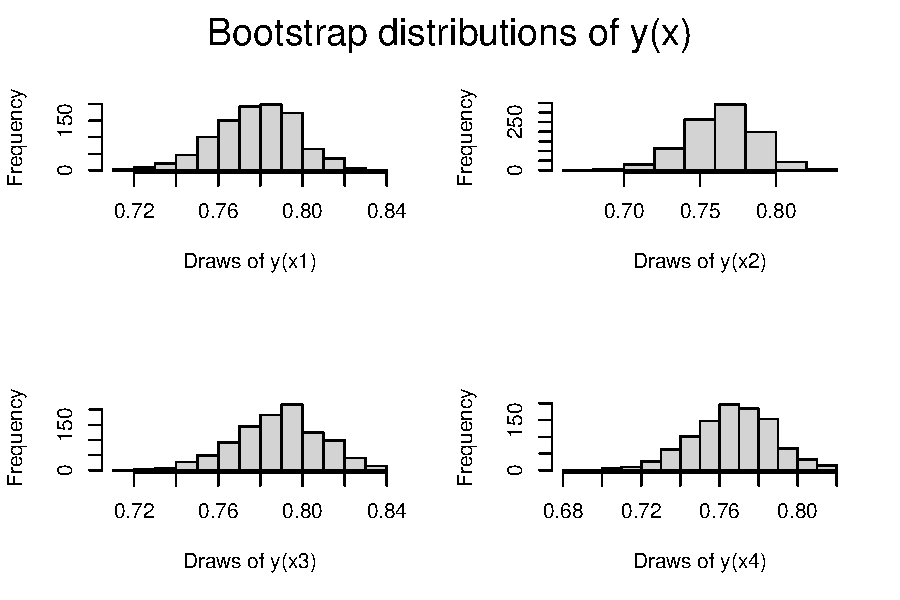
\includegraphics{fig-ds/bootstrap.pdf}
 \caption{Bootstrap distributions for $4$ randomly chosen inputs, $\bx_i$, $i = 1, 2, 3, 4$, from the wave $2$ design. The bootstrap distribution for $y(\bx_i)$ is based on $1000$ values of $y(\bx_i)$. \label{Fig:bootstrap}}
\end{figure}
The bootstrap distributions shown in \cref{Fig:bootstrap} all support the assumption that $y(\bx)$ is unimodal, even though $u(\bx_i)$ has a multimodal distribution. Note that, if $y(\bx)$ was still multimodal, the methodology we used would not work. To remedy this, we can increase the sample size which $y(\bx)$ are based on. This will mean that training data are more expensive to obtain; the benefit is that we can avoid many awkward probability distributions and thus utilise relatively simple and robust methods to quantity uncertainty about $U(\bx)$.
\subsubsection{Consistency of final NROY volume}
To check that the final NROY volume is indeed consistent with our uncertainty about the optimal decision, we can re-use the large samples presented in \cref{Fig:final-avail}. In particular, the $300$ samples shown in each sub-figure are random draws which are independent of any emulator training data and the emulators themselves. The means and standard errors implied by these samples offer an independent perspective of $U(\bx)$ for each $\bx$. Comparing these to the emulator's characterisation of $U(\hat{\bx}_2)$ allows us to assess if the apparently NROY decisions should have been ruled out.
\begin{table}
\centering
\begin{tabular}{rrrr}
 \toprule
 Decision & $\widehat{U}(\bx)$ & $\widehat{\text{s.e.}}(\bx)$ & $I^{*}(\bx)$ \\\cmidrule{1-4}
 1 & $0.788$ & $5.592\times 10^{-3}$ & $1.801$ \\
  2 & $0.786$ & $6.138\times 10^{-3}$ & $1.897$ \\
  3 & $0.806$ & $6.254\times 10^{-3}$ & $0.739$ \\
  4 & $0.797$ & $5.832\times 10^{-3}$ & $1.281$ \\
  5 & $0.793$ & $6.326\times 10^{-3}$ & $1.484$ \\
  6 & $0.800$ & $5.414\times 10^{-3}$ & $1.071$ \\
  7 & $0.789$ & $6.244\times 10^{-3}$ & $1.728$ \\
  8 & $0.801$ & $5.657\times 10^{-3}$ & $1.053$ \\
  9 & $0.799$ & $5.978\times 10^{-3}$ & $1.139$ \\
  10 & $0.791$ & $6.406\times 10^{-3}$ & $1.614$ \\
  11 & $0.807$ & $5.708\times 10^{-3}$ & $0.693$ \\
  12 & $0.788$ & $6.317\times 10^{-3}$ & $1.797$ \\\bottomrule
\end{tabular}
\caption{Means ($\widehat{U}$) and standard errors ($\widehat{\text{s.e.}}$) for the expected utility of the $12$ decisions corresponding to \cref{Fig:final-avail} and \cref{Tab:final-dec}, as well as an implausibility measure ($I^{*}$) for each decision. \label{Tab:final-dec-implaus} }
\end{table}
\cref{Tab:final-dec-implaus} shows the mean and standard error for each of the $6$ decisions given in \cref{Fig:final-avail}. Our implausibility measure for this final aspect of the analysis will be
\begin{equation}
 I^{*}(\bx) = \frac{\E\{U(\hat{\bx}_1)\} - \hat{U}(\bx_i) }{ \sqrt{ \var\{U(\hat{\bx}_1)\} + \widehat{ \text{s.e.} }\{\hat{U}(\bx_i)\}^2 }\ }
\end{equation}
where $\widehat{ \text{s.e.} }\{\hat{U}(\bx_i)\}$ is the estimated standard error of $\hat{U}(\bx_i)$. Recall that $\bx_6 = \hat{\bx}_2$. In this case we see that $0$ decisions are ruled out under $I^{*}$. Under Pukelsheim's $3\sigma$ rule we would expect to retain \textit{at least} $90\%$ of decisions after two well-calibrated waves. Assuming Normality (and a cut off of $3$) we would expect to retain around $98\%$ of decisions after two well-calibrated waves. This sample size is small but $100\%$ is close enough to $98\%$, and clearly $100\% > 90\%$, we therefore judge that our ruling out procedure is well-calibrated.

\section{Discussion}

We have presented a history matching inspired procedure for decision support with the stochastic Athena simulator. Our approach drew on established ideas, such as the UCB BayesOpt heuristic \citep{Srinivas2009} and history-matching inspired decision support for deterministic simulators \citep{Owen2020} but relied on novel applications of these ideas to address the challenges within our applied problem of decision support under uncertainty for the Athena simulator.

We first provided an illustrative elicitation of a utility function. We drew on key attributes to the problem, but we stress the elicitation will always be subjective; every DM has their own utility function.

We then proposed unifying two established approaches. We began by performing three independent rounds of BayesOpt to optimise the choices of $x_1$--$x_{18}$ then used techniques from the HM literature to communicate uncertainty about the optimal decision. Our HM inspired approach required a novel implausibility measure which accounts for dependence across the decision space.

We then considered the design for our decision support exercise. Since a subset of our inputs were a discrete simplex, which is non-standard in the computer experiments literature, this posed some interesting challenges. BayesOpt allowed us to side-step the problem of design for a wave $1$ emulator since it automatically chooses where to run the simulator. The design for a wave $2$ emulator was more challenging as we had to adhere to the constraints of the decision task a whilst constructing a design within the NROY region that provided a diverse set of decisions. Sequential design offered a promising approach again. Our approximate ALM design allowed us to construct a design which was more space-filling than a uniform design. We believe sequential designs are a promising option for non-standard input spaces.

We then constructed a new pair of emulators to further explore the NROY space. We performed a sensitivity analysis based on the choice of possible maxima. One maximum led to a negligible reduction in the NROY space and the other led to a small reduction in the NROY space. In general, we would advise using the results of the most recent emulator to choose the maximiser (when $y(\bx)$ is stochastic). This would protect against $U(\hat{\bx})$ being an over-estimate, which may rule out too many decisions. In the deterministic case, it would be natural to choose the largest observed value across all waves.

Next we presented the DM with a set of sensible decisions that could be taken. We presented decisions from both warehouses and from diverse decisions within each warehouse.

Finally, we performed some post-hoc checks to verify some assumptions, as well as checking whether the proportion of incorrectly ruled out decisions is consistent with Pukelsheim's $3\sigma$ rule. Our small sample of decisions suggested that we did not rule out too many decisions, although a much larger sample would be needed to make a conclusive statement.

If we were to perform the analysis again, with the assistance of a DM, we could prevent ruling out too many decisions by incorporating model discrepancy. It would be possible to estimate model discrepancy via the elicitation procedure. When fitting the utility function to the DM's beliefs, we could use the `over-fitting' technique in which we elicit more preferences than necessary. We can then fit a functional form to the elicited quantities via least squares. The sum of squares will be positive and can be interpreted as a variance. This sum of squares can be used as a \textit{minimum} model discrepancy. Nonetheless, even if we did rule out too many decisions, commonly used approaches would have only provided one decision. Thus, we have been successful in \textit{supporting} decision making, rather than making the decision on behalf of the DM.

Another avenue for further investigation would be simulation experiments to learn about various aspects of our approach. \correction{Firstly, we are not aware of any simulation experiments which address how often a history matching based approach will rule out the `true' maximiser. In part, this gap in the literature will be due to the complexities of HM. Describing an NROY region is only practically possible by testing whether points are in the NROY region or not.  We do not consider this to be a problem for this work as HM delivers what we need: a greatly reduced decision space from which a DM can choose a good --- not necessarily optimal --- decision.}

Another aspect which would benefit from further investigation would be the choice of design. We pragmatically chose to use an ALM design based on (a) the range of the NROY volume covered by the design and (b) the theory behind ALM designs which suggests points should be spread apart, so we are considering `diverse' decisions. It would be interesting to see if there is any \textit{numerical} evidence to suggest that this approach is better, or indeed, worse than other methods. We would also like to investigate whether integrating the BayesOpt routine improved the history matching inspired approach. This would be in contrast to \citet{Owen2020} who used one shot designs for every wave of emulation, including the first, which may have allowed for greater exploration.

In terms of the decision problem, we considered a static policy in the sense that the decision variables do not change with time. However, many approaches within \citet{Tusar2022} were dynamic policies. We could consider two forms of dynamic policy: those which change with time, or those which change as data arrives (for example, updating prior beliefs with data, then maximising the DM's utility function with respect to a posterior distribution). A dynamic policy is where $\bx$ is replaced with $\bx(t)$, a vector-valued function of time. If $\bx$ is replaced by $\bx(t)$, the decision problem could be of a much higher dimension than our problem which has $17$ degrees of freedom. HM is an effective approach even in very high dimensional settings, for example \citet{White2018} uses HM to find plausible values for around $2500$ inputs. We imagine the methodology used in this chapter and used by \citet{Lawson2016} and \citet{Owen2020} could be successfully applied in other high dimensional settings. If the policy is dynamic in the sense that beliefs are being updated constantly or periodically, we would use exactly the same approach as above, with the addition that the procedure is run according to a pre-defined schedule. This would allow the DM to revise their utility function if aspects of the problem had changed. For example, the Athena simulator could be revised to offer an improved reflection of reality, or the DM may wish to update their utility function to incorporate new concerns. A dynamic policy however may not be suited to warehouse choice, but rather updating how we run a given warehouse.
\end{chapter}
